\chapter{Sterowanie rzeczywistym obiektem - część laboratoryjna}

Zadanie laboratoryjne polegało na zebraniu danych z rzeczywistego obiektu oraz implementacji na nim algorytmów regulacji PID i DMC. Badanym obiektem było stanowisko grzewczo-chłodzące. Obiekt ten charakteryzuje się opóźnieniem na wejściu oraz wolną dynamiką. Taka charakterystyka obiektu ma znaczący wpływ na jakość danych regulatorów.

Do zadania sterowania, jako wejście posłużyła moc grzałki sterowana w granicach 0-100\% (G1), wyjściem była temperatura mierzona przy grzałce (T1). Dodatkowo zostało wprowadzone stałe zakłócenie w postaci wentylatora (W1) któego moc była ustawiona na 50\% (traktowane jako cecha otoczenia).

\section{Odpowiedzi skokowe}
Pierwszą częścią zadania było pobranie odpowiedzi skokowych z obiektu zaczynając z ustalonego punktu pracy. Wybranym przez nas puktem pracy było $U_\mathrm{pp}=0$. Dla takiej wartości, wartość wyjścia w punkcie pracy wynosiła około $Y_\mathrm{pp}=24$. Wykonano 3 eksperymenty dla różnych skoków sterowania. Ich efekty przedstawione są na Rys.~\ref{w1}

\begin{figure}

\centering
\caption{ }
% This file was created by matlab2tikz.
%
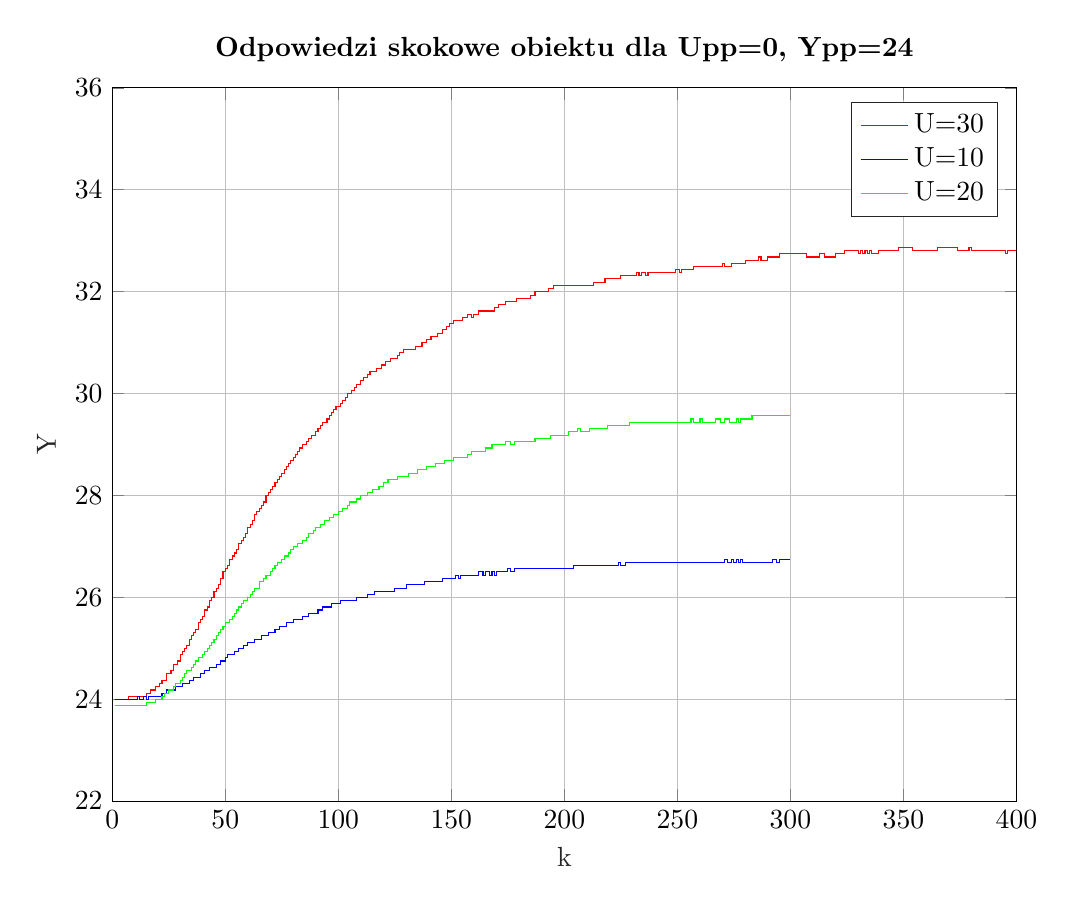
\begin{tikzpicture}

\begin{axis}[%
width=4.521in,
height=3.566in,
at={(0.758in,0.481in)},
scale only axis,
xmin=0,
xmax=400,
xlabel style={font=\color{white!15!black}},
xlabel={k},
ymin=22,
ymax=36,
ylabel style={font=\color{white!15!black}},
ylabel={Y},
axis background/.style={fill=white},
title style={font=\bfseries},
title={Odpowiedzi skokowe obiektu dla Upp=0, Ypp=24},
xmajorgrids,
ymajorgrids,
legend style={legend cell align=left, align=left, draw=white!15!black}
]
\addplot[const plot, color=red] table[row sep=crcr] {%
1	24\\
2	24\\
3	24\\
4	24\\
5	24\\
6	24\\
7	24.06\\
8	24.06\\
9	24.06\\
10	24.06\\
11	24.06\\
12	24.06\\
13	24.06\\
14	24.06\\
15	24.12\\
16	24.12\\
17	24.18\\
18	24.18\\
19	24.25\\
20	24.25\\
21	24.31\\
22	24.37\\
23	24.37\\
24	24.5\\
25	24.5\\
26	24.56\\
27	24.68\\
28	24.68\\
29	24.75\\
30	24.87\\
31	24.93\\
32	25\\
33	25.06\\
34	25.18\\
35	25.25\\
36	25.31\\
37	25.37\\
38	25.5\\
39	25.56\\
40	25.62\\
41	25.75\\
42	25.81\\
43	25.93\\
44	26\\
45	26.12\\
46	26.18\\
47	26.25\\
48	26.37\\
49	26.5\\
50	26.56\\
51	26.62\\
52	26.75\\
53	26.81\\
54	26.87\\
55	26.93\\
56	27.06\\
57	27.12\\
58	27.18\\
59	27.25\\
60	27.37\\
61	27.43\\
62	27.5\\
63	27.62\\
64	27.68\\
65	27.75\\
66	27.81\\
67	27.87\\
68	28\\
69	28.06\\
70	28.12\\
71	28.18\\
72	28.25\\
73	28.31\\
74	28.37\\
75	28.43\\
76	28.5\\
77	28.56\\
78	28.62\\
79	28.68\\
80	28.75\\
81	28.81\\
82	28.87\\
83	28.93\\
84	29\\
85	29\\
86	29.06\\
87	29.12\\
88	29.18\\
89	29.18\\
90	29.25\\
91	29.31\\
92	29.37\\
93	29.43\\
94	29.43\\
95	29.5\\
96	29.56\\
97	29.62\\
98	29.68\\
99	29.75\\
100	29.75\\
101	29.81\\
102	29.87\\
103	29.93\\
104	30\\
105	30\\
106	30.06\\
107	30.12\\
108	30.18\\
109	30.18\\
110	30.25\\
111	30.31\\
112	30.31\\
113	30.37\\
114	30.43\\
115	30.43\\
116	30.43\\
117	30.5\\
118	30.5\\
119	30.56\\
120	30.56\\
121	30.62\\
122	30.62\\
123	30.68\\
124	30.68\\
125	30.68\\
126	30.75\\
127	30.81\\
128	30.81\\
129	30.87\\
130	30.87\\
131	30.87\\
132	30.87\\
133	30.87\\
134	30.93\\
135	30.93\\
136	30.93\\
137	31\\
138	31\\
139	31.06\\
140	31.06\\
141	31.12\\
142	31.12\\
143	31.12\\
144	31.18\\
145	31.18\\
146	31.25\\
147	31.25\\
148	31.31\\
149	31.37\\
150	31.37\\
151	31.43\\
152	31.43\\
153	31.43\\
154	31.43\\
155	31.5\\
156	31.5\\
157	31.56\\
158	31.56\\
159	31.5\\
160	31.56\\
161	31.56\\
162	31.62\\
163	31.62\\
164	31.62\\
165	31.62\\
166	31.62\\
167	31.62\\
168	31.62\\
169	31.68\\
170	31.68\\
171	31.75\\
172	31.75\\
173	31.75\\
174	31.81\\
175	31.81\\
176	31.81\\
177	31.81\\
178	31.81\\
179	31.87\\
180	31.87\\
181	31.87\\
182	31.87\\
183	31.87\\
184	31.87\\
185	31.93\\
186	31.93\\
187	32\\
188	32\\
189	32\\
190	32\\
191	32\\
192	32\\
193	32.06\\
194	32.06\\
195	32.12\\
196	32.12\\
197	32.12\\
198	32.12\\
199	32.12\\
200	32.12\\
201	32.12\\
202	32.12\\
203	32.12\\
204	32.12\\
205	32.12\\
206	32.12\\
207	32.12\\
208	32.12\\
209	32.12\\
210	32.12\\
211	32.12\\
212	32.12\\
213	32.18\\
214	32.18\\
215	32.18\\
216	32.18\\
217	32.18\\
218	32.25\\
219	32.25\\
220	32.25\\
221	32.25\\
222	32.25\\
223	32.25\\
224	32.25\\
225	32.31\\
226	32.31\\
227	32.31\\
228	32.31\\
229	32.31\\
230	32.31\\
231	32.31\\
232	32.37\\
233	32.31\\
234	32.37\\
235	32.37\\
236	32.31\\
237	32.37\\
238	32.37\\
239	32.37\\
240	32.37\\
241	32.37\\
242	32.37\\
243	32.37\\
244	32.37\\
245	32.37\\
246	32.37\\
247	32.37\\
248	32.37\\
249	32.43\\
250	32.43\\
251	32.37\\
252	32.43\\
253	32.43\\
254	32.43\\
255	32.43\\
256	32.43\\
257	32.5\\
258	32.5\\
259	32.5\\
260	32.5\\
261	32.5\\
262	32.5\\
263	32.5\\
264	32.5\\
265	32.5\\
266	32.5\\
267	32.5\\
268	32.5\\
269	32.5\\
270	32.56\\
271	32.5\\
272	32.5\\
273	32.5\\
274	32.56\\
275	32.56\\
276	32.56\\
277	32.56\\
278	32.56\\
279	32.56\\
280	32.62\\
281	32.62\\
282	32.62\\
283	32.62\\
284	32.62\\
285	32.62\\
286	32.68\\
287	32.62\\
288	32.62\\
289	32.62\\
290	32.68\\
291	32.68\\
292	32.68\\
293	32.68\\
294	32.68\\
295	32.75\\
296	32.75\\
297	32.75\\
298	32.75\\
299	32.75\\
300	32.75\\
301	32.75\\
302	32.75\\
303	32.75\\
304	32.75\\
305	32.75\\
306	32.75\\
307	32.68\\
308	32.68\\
309	32.68\\
310	32.68\\
311	32.68\\
312	32.68\\
313	32.75\\
314	32.75\\
315	32.68\\
316	32.68\\
317	32.68\\
318	32.68\\
319	32.68\\
320	32.75\\
321	32.75\\
322	32.75\\
323	32.75\\
324	32.81\\
325	32.81\\
326	32.81\\
327	32.81\\
328	32.81\\
329	32.81\\
330	32.75\\
331	32.81\\
332	32.75\\
333	32.81\\
334	32.75\\
335	32.81\\
336	32.75\\
337	32.75\\
338	32.75\\
339	32.81\\
340	32.81\\
341	32.81\\
342	32.81\\
343	32.81\\
344	32.81\\
345	32.81\\
346	32.81\\
347	32.81\\
348	32.87\\
349	32.87\\
350	32.87\\
351	32.87\\
352	32.87\\
353	32.87\\
354	32.81\\
355	32.81\\
356	32.81\\
357	32.81\\
358	32.81\\
359	32.81\\
360	32.81\\
361	32.81\\
362	32.81\\
363	32.81\\
364	32.81\\
365	32.87\\
366	32.87\\
367	32.87\\
368	32.87\\
369	32.87\\
370	32.87\\
371	32.87\\
372	32.87\\
373	32.87\\
374	32.81\\
375	32.81\\
376	32.81\\
377	32.81\\
378	32.81\\
379	32.87\\
380	32.81\\
381	32.81\\
382	32.81\\
383	32.81\\
384	32.81\\
385	32.81\\
386	32.81\\
387	32.81\\
388	32.81\\
389	32.81\\
390	32.81\\
391	32.81\\
392	32.81\\
393	32.81\\
394	32.81\\
395	32.75\\
396	32.81\\
397	32.81\\
398	32.81\\
399	32.81\\
400	32.81\\
401	32.81\\
402	32.81\\
403	32.87\\
404	32.81\\
405	32.87\\
406	32.87\\
407	32.87\\
408	32.87\\
409	32.87\\
410	32.81\\
411	32.81\\
412	32.81\\
413	32.81\\
414	32.81\\
415	32.81\\
416	32.81\\
417	32.81\\
418	32.81\\
419	32.81\\
420	32.81\\
421	32.81\\
422	32.81\\
423	32.81\\
424	32.81\\
425	32.81\\
426	32.81\\
427	32.81\\
428	32.81\\
429	32.81\\
430	32.81\\
431	32.81\\
432	32.75\\
433	32.81\\
434	32.81\\
435	32.81\\
436	32.81\\
437	32.81\\
438	32.81\\
439	32.81\\
440	32.75\\
441	32.75\\
442	32.75\\
443	32.75\\
444	32.75\\
445	32.75\\
446	32.75\\
447	32.75\\
448	32.75\\
449	32.75\\
450	32.81\\
451	32.81\\
452	32.81\\
453	32.87\\
454	32.87\\
455	32.87\\
456	32.93\\
457	32.93\\
458	32.87\\
459	32.87\\
460	32.87\\
461	32.87\\
462	32.87\\
463	32.93\\
464	32.87\\
465	32.87\\
466	32.93\\
467	32.93\\
468	32.93\\
469	32.93\\
470	32.93\\
471	32.93\\
472	32.93\\
473	32.93\\
474	33\\
475	33\\
476	33\\
477	32.93\\
478	33\\
479	32.93\\
480	32.93\\
481	32.93\\
482	33\\
483	33\\
484	32.93\\
485	32.93\\
486	33\\
487	32.93\\
488	32.93\\
489	32.93\\
490	32.93\\
491	32.87\\
492	32.93\\
493	32.87\\
494	32.87\\
495	32.87\\
496	32.87\\
497	32.87\\
498	32.87\\
499	32.87\\
500	32.87\\
501	32.87\\
502	32.87\\
503	32.81\\
504	32.87\\
505	32.87\\
506	32.87\\
507	32.87\\
508	32.87\\
509	32.87\\
510	32.87\\
511	32.87\\
512	32.87\\
513	32.87\\
514	32.87\\
515	32.87\\
516	32.87\\
517	32.87\\
518	32.87\\
519	32.87\\
520	32.87\\
521	32.93\\
522	32.93\\
523	32.93\\
524	32.93\\
525	32.93\\
526	33\\
527	33\\
528	33\\
529	33\\
530	33.06\\
531	33.06\\
532	33.06\\
533	33.06\\
534	33.06\\
535	33.06\\
536	33.06\\
537	33.06\\
538	33.12\\
539	33.12\\
540	33.12\\
541	33.12\\
542	33.12\\
543	33.12\\
544	33.12\\
545	33.12\\
546	33.12\\
547	33.12\\
548	33.12\\
549	33.12\\
550	33.12\\
551	33.12\\
552	33.12\\
553	33.12\\
554	33.12\\
555	33.18\\
556	33.12\\
557	33.12\\
558	33.12\\
559	33.12\\
560	33.12\\
561	33.12\\
562	33.06\\
563	33.06\\
564	33.06\\
565	33.06\\
566	33.06\\
567	33.06\\
568	33.12\\
569	33.12\\
570	33.12\\
571	33.12\\
572	33.12\\
573	33.12\\
574	33.12\\
575	33.12\\
576	33.12\\
577	33.18\\
578	33.18\\
579	33.18\\
580	33.18\\
581	33.25\\
582	33.25\\
583	33.25\\
584	33.18\\
585	33.25\\
586	33.18\\
587	33.18\\
588	33.18\\
589	33.18\\
590	33.25\\
591	33.18\\
592	33.18\\
593	33.12\\
594	33.18\\
595	33.18\\
596	33.18\\
597	33.18\\
598	33.18\\
599	33.18\\
600	33.18\\
};
\addlegendentry{U=30}

\addplot[const plot, color=blue] table[row sep=crcr] {%
1	24\\
2	24\\
3	24\\
4	24\\
5	24\\
6	24\\
7	24\\
8	24\\
9	24\\
10	24\\
11	24.06\\
12	24\\
13	24\\
14	24.06\\
15	24\\
16	24.06\\
17	24.06\\
18	24.06\\
19	24.06\\
20	24.06\\
21	24.06\\
22	24.12\\
23	24.12\\
24	24.18\\
25	24.18\\
26	24.18\\
27	24.18\\
28	24.25\\
29	24.25\\
30	24.25\\
31	24.31\\
32	24.31\\
33	24.31\\
34	24.37\\
35	24.37\\
36	24.43\\
37	24.43\\
38	24.43\\
39	24.5\\
40	24.5\\
41	24.56\\
42	24.56\\
43	24.62\\
44	24.62\\
45	24.62\\
46	24.68\\
47	24.68\\
48	24.75\\
49	24.75\\
50	24.81\\
51	24.87\\
52	24.87\\
53	24.87\\
54	24.93\\
55	24.93\\
56	25\\
57	25\\
58	25.06\\
59	25.06\\
60	25.12\\
61	25.12\\
62	25.12\\
63	25.18\\
64	25.18\\
65	25.18\\
66	25.25\\
67	25.25\\
68	25.25\\
69	25.31\\
70	25.31\\
71	25.31\\
72	25.37\\
73	25.37\\
74	25.43\\
75	25.43\\
76	25.43\\
77	25.5\\
78	25.5\\
79	25.5\\
80	25.56\\
81	25.56\\
82	25.56\\
83	25.56\\
84	25.62\\
85	25.62\\
86	25.62\\
87	25.68\\
88	25.68\\
89	25.68\\
90	25.68\\
91	25.75\\
92	25.75\\
93	25.81\\
94	25.81\\
95	25.81\\
96	25.81\\
97	25.87\\
98	25.87\\
99	25.87\\
100	25.87\\
101	25.93\\
102	25.93\\
103	25.93\\
104	25.93\\
105	25.93\\
106	25.93\\
107	25.93\\
108	26\\
109	26\\
110	26\\
111	26\\
112	26\\
113	26.06\\
114	26.06\\
115	26.06\\
116	26.12\\
117	26.12\\
118	26.12\\
119	26.12\\
120	26.12\\
121	26.12\\
122	26.12\\
123	26.12\\
124	26.12\\
125	26.18\\
126	26.18\\
127	26.18\\
128	26.18\\
129	26.18\\
130	26.25\\
131	26.25\\
132	26.25\\
133	26.25\\
134	26.25\\
135	26.25\\
136	26.25\\
137	26.25\\
138	26.31\\
139	26.31\\
140	26.31\\
141	26.31\\
142	26.31\\
143	26.31\\
144	26.31\\
145	26.31\\
146	26.37\\
147	26.37\\
148	26.37\\
149	26.37\\
150	26.37\\
151	26.37\\
152	26.43\\
153	26.37\\
154	26.43\\
155	26.43\\
156	26.43\\
157	26.43\\
158	26.43\\
159	26.43\\
160	26.43\\
161	26.43\\
162	26.5\\
163	26.5\\
164	26.43\\
165	26.5\\
166	26.5\\
167	26.43\\
168	26.5\\
169	26.43\\
170	26.5\\
171	26.5\\
172	26.5\\
173	26.5\\
174	26.5\\
175	26.56\\
176	26.5\\
177	26.5\\
178	26.56\\
179	26.56\\
180	26.56\\
181	26.56\\
182	26.56\\
183	26.56\\
184	26.56\\
185	26.56\\
186	26.56\\
187	26.56\\
188	26.56\\
189	26.56\\
190	26.56\\
191	26.56\\
192	26.56\\
193	26.56\\
194	26.56\\
195	26.56\\
196	26.56\\
197	26.56\\
198	26.56\\
199	26.56\\
200	26.56\\
201	26.56\\
202	26.56\\
203	26.56\\
204	26.62\\
205	26.62\\
206	26.62\\
207	26.62\\
208	26.62\\
209	26.62\\
210	26.62\\
211	26.62\\
212	26.62\\
213	26.62\\
214	26.62\\
215	26.62\\
216	26.62\\
217	26.62\\
218	26.62\\
219	26.62\\
220	26.62\\
221	26.62\\
222	26.62\\
223	26.62\\
224	26.68\\
225	26.62\\
226	26.62\\
227	26.68\\
228	26.68\\
229	26.68\\
230	26.68\\
231	26.68\\
232	26.68\\
233	26.68\\
234	26.68\\
235	26.68\\
236	26.68\\
237	26.68\\
238	26.68\\
239	26.68\\
240	26.68\\
241	26.68\\
242	26.68\\
243	26.68\\
244	26.68\\
245	26.68\\
246	26.68\\
247	26.68\\
248	26.68\\
249	26.68\\
250	26.68\\
251	26.68\\
252	26.68\\
253	26.68\\
254	26.68\\
255	26.68\\
256	26.68\\
257	26.68\\
258	26.68\\
259	26.68\\
260	26.68\\
261	26.68\\
262	26.68\\
263	26.68\\
264	26.68\\
265	26.68\\
266	26.68\\
267	26.68\\
268	26.68\\
269	26.68\\
270	26.68\\
271	26.75\\
272	26.68\\
273	26.68\\
274	26.75\\
275	26.68\\
276	26.75\\
277	26.68\\
278	26.75\\
279	26.68\\
280	26.68\\
281	26.68\\
282	26.68\\
283	26.68\\
284	26.68\\
285	26.68\\
286	26.68\\
287	26.68\\
288	26.68\\
289	26.68\\
290	26.68\\
291	26.68\\
292	26.75\\
293	26.75\\
294	26.68\\
295	26.75\\
296	26.75\\
297	26.75\\
298	26.75\\
299	26.75\\
300	26.75\\
};
\addlegendentry{U=10}

\addplot[const plot, color=green] table[row sep=crcr] {%
1	23.87\\
2	23.87\\
3	23.87\\
4	23.87\\
5	23.87\\
6	23.87\\
7	23.87\\
8	23.87\\
9	23.87\\
10	23.87\\
11	23.87\\
12	23.87\\
13	23.87\\
14	23.87\\
15	23.93\\
16	23.93\\
17	23.93\\
18	23.93\\
19	24\\
20	24\\
21	24\\
22	24.06\\
23	24.12\\
24	24.12\\
25	24.18\\
26	24.18\\
27	24.25\\
28	24.31\\
29	24.31\\
30	24.37\\
31	24.43\\
32	24.5\\
33	24.56\\
34	24.56\\
35	24.62\\
36	24.68\\
37	24.75\\
38	24.81\\
39	24.81\\
40	24.87\\
41	24.93\\
42	25\\
43	25.06\\
44	25.12\\
45	25.18\\
46	25.25\\
47	25.31\\
48	25.37\\
49	25.43\\
50	25.5\\
51	25.5\\
52	25.56\\
53	25.62\\
54	25.68\\
55	25.75\\
56	25.81\\
57	25.87\\
58	25.93\\
59	25.93\\
60	26\\
61	26.06\\
62	26.12\\
63	26.18\\
64	26.18\\
65	26.31\\
66	26.31\\
67	26.37\\
68	26.43\\
69	26.43\\
70	26.5\\
71	26.56\\
72	26.62\\
73	26.68\\
74	26.68\\
75	26.75\\
76	26.81\\
77	26.81\\
78	26.87\\
79	26.93\\
80	27\\
81	27\\
82	27.06\\
83	27.06\\
84	27.12\\
85	27.12\\
86	27.18\\
87	27.25\\
88	27.25\\
89	27.31\\
90	27.37\\
91	27.37\\
92	27.43\\
93	27.43\\
94	27.5\\
95	27.5\\
96	27.56\\
97	27.56\\
98	27.62\\
99	27.62\\
100	27.68\\
101	27.68\\
102	27.75\\
103	27.75\\
104	27.81\\
105	27.87\\
106	27.87\\
107	27.87\\
108	27.93\\
109	27.93\\
110	28\\
111	28\\
112	28\\
113	28.06\\
114	28.06\\
115	28.12\\
116	28.12\\
117	28.12\\
118	28.18\\
119	28.18\\
120	28.25\\
121	28.25\\
122	28.31\\
123	28.31\\
124	28.31\\
125	28.31\\
126	28.37\\
127	28.37\\
128	28.37\\
129	28.37\\
130	28.37\\
131	28.43\\
132	28.43\\
133	28.43\\
134	28.43\\
135	28.5\\
136	28.5\\
137	28.5\\
138	28.5\\
139	28.56\\
140	28.56\\
141	28.56\\
142	28.56\\
143	28.62\\
144	28.62\\
145	28.62\\
146	28.62\\
147	28.68\\
148	28.68\\
149	28.68\\
150	28.68\\
151	28.75\\
152	28.75\\
153	28.75\\
154	28.75\\
155	28.75\\
156	28.75\\
157	28.81\\
158	28.81\\
159	28.87\\
160	28.87\\
161	28.87\\
162	28.87\\
163	28.87\\
164	28.87\\
165	28.93\\
166	28.93\\
167	28.93\\
168	29\\
169	29\\
170	29\\
171	29\\
172	29\\
173	29\\
174	29.06\\
175	29.06\\
176	29\\
177	29\\
178	29.06\\
179	29.06\\
180	29.06\\
181	29.06\\
182	29.06\\
183	29.06\\
184	29.06\\
185	29.06\\
186	29.06\\
187	29.12\\
188	29.12\\
189	29.12\\
190	29.12\\
191	29.12\\
192	29.12\\
193	29.12\\
194	29.18\\
195	29.18\\
196	29.18\\
197	29.18\\
198	29.18\\
199	29.18\\
200	29.18\\
201	29.18\\
202	29.25\\
203	29.25\\
204	29.25\\
205	29.25\\
206	29.31\\
207	29.25\\
208	29.25\\
209	29.25\\
210	29.25\\
211	29.31\\
212	29.31\\
213	29.31\\
214	29.31\\
215	29.31\\
216	29.31\\
217	29.31\\
218	29.31\\
219	29.37\\
220	29.37\\
221	29.37\\
222	29.37\\
223	29.37\\
224	29.37\\
225	29.37\\
226	29.37\\
227	29.37\\
228	29.37\\
229	29.43\\
230	29.43\\
231	29.43\\
232	29.43\\
233	29.43\\
234	29.43\\
235	29.43\\
236	29.43\\
237	29.43\\
238	29.43\\
239	29.43\\
240	29.43\\
241	29.43\\
242	29.43\\
243	29.43\\
244	29.43\\
245	29.43\\
246	29.43\\
247	29.43\\
248	29.43\\
249	29.43\\
250	29.43\\
251	29.43\\
252	29.43\\
253	29.43\\
254	29.43\\
255	29.43\\
256	29.5\\
257	29.43\\
258	29.43\\
259	29.43\\
260	29.5\\
261	29.43\\
262	29.43\\
263	29.43\\
264	29.43\\
265	29.43\\
266	29.43\\
267	29.5\\
268	29.5\\
269	29.43\\
270	29.43\\
271	29.5\\
272	29.5\\
273	29.43\\
274	29.43\\
275	29.43\\
276	29.5\\
277	29.43\\
278	29.5\\
279	29.5\\
280	29.5\\
281	29.5\\
282	29.5\\
283	29.56\\
284	29.56\\
285	29.56\\
286	29.56\\
287	29.56\\
288	29.56\\
289	29.56\\
290	29.56\\
291	29.56\\
292	29.56\\
293	29.56\\
294	29.56\\
295	29.56\\
296	29.56\\
297	29.56\\
298	29.56\\
299	29.56\\
300	29.56\\
};
\addlegendentry{U=20}

\end{axis}
\end{tikzpicture}%
\label{w1}
\end{figure}

Doświadczenie dla $U=30$ zostało przeprowadzone na dłuższej próbie czasowej ze względu na dłuższy czas ustalenia się wyjścia obiektu dla zadanego sterowania. Już na pierwszy rzut oka można stwierdzić, że obiekt ten jest liniowy co potwierdza tylko jego charakterystyka statyczna przedstawiona na Rys.~{w2}. Tak zebrane odpowiedzi skokowe posłużyły następnie do wyznaczenia dopowiedzi skokowej dla skoku jendostkowego (przedstawiona na Rys.~{w3}), która następnie posłużyła do implementacji algorytmu DMC.

\begin{figure}

\centering
\caption{}
% This file was created by matlab2tikz.
%
\definecolor{mycolor1}{rgb}{0.00000,0.44700,0.74100}%
%
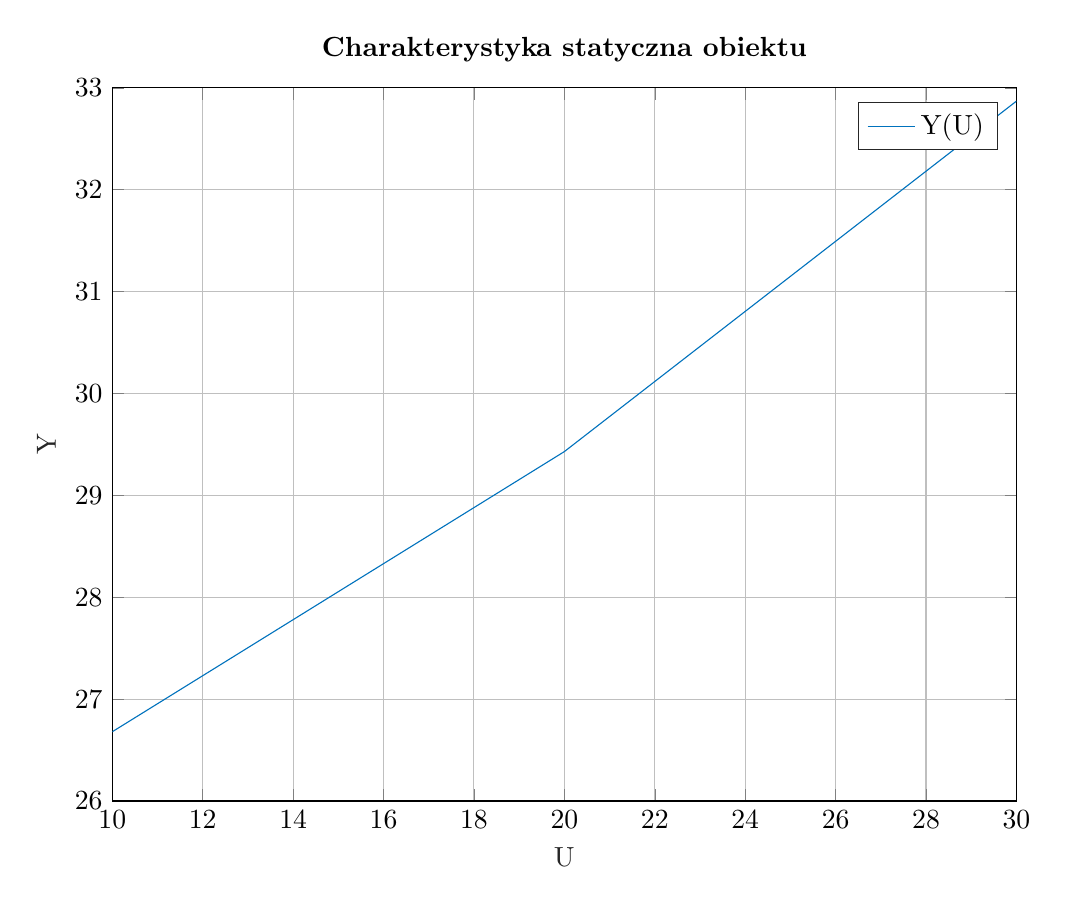
\begin{tikzpicture}

\begin{axis}[%
width=4.521in,
height=3.566in,
at={(0.758in,0.481in)},
scale only axis,
xmin=10,
xmax=30,
xlabel style={font=\color{white!15!black}},
xlabel={U},
ymin=26,
ymax=33,
ylabel style={font=\color{white!15!black}},
ylabel={Y},
axis background/.style={fill=white},
title style={font=\bfseries},
title={Charakterystyka statyczna obiektu},
xmajorgrids,
ymajorgrids,
legend style={legend cell align=left, align=left, draw=white!15!black}
]
\addplot [color=mycolor1]
  table[row sep=crcr]{%
10	26.68\\
20	29.43\\
30	32.87\\
};
\addlegendentry{Y(U)}

\end{axis}
\end{tikzpicture}%
\label{w2}
\end{figure}

\begin{figure}

	\centering
	\caption{ }
	% This file was created by matlab2tikz.
%
\definecolor{mycolor1}{rgb}{0.00000,0.44700,0.74100}%
%
\begin{tikzpicture}

\begin{axis}[%
width=4.521in,
height=3.566in,
at={(0.758in,0.481in)},
scale only axis,
xmin=0,
xmax=400,
xlabel style={font=\color{white!15!black}},
xlabel={k},
ymin=0,
ymax=0.3,
ylabel style={font=\color{white!15!black}},
ylabel={Y},
axis background/.style={fill=white},
title style={font=\bfseries},
title={Przekszta�cona odpowied� skokowa obiektu},
xmajorgrids,
ymajorgrids,
legend style={legend cell align=left, align=left, draw=white!15!black}
]
\addplot[const plot, color=mycolor1] table[row sep=crcr] {%
1	0\\
2	0\\
3	0\\
4	0\\
5	0\\
6	0\\
7	0.00199999999999989\\
8	0.00199999999999989\\
9	0.00199999999999989\\
10	0.00199999999999989\\
11	0.00199999999999989\\
12	0.00199999999999989\\
13	0.00199999999999989\\
14	0.00199999999999989\\
15	0.004\\
16	0.004\\
17	0.00599999999999989\\
18	0.00599999999999989\\
19	0.0083333333333333\\
20	0.0083333333333333\\
21	0.0103333333333332\\
22	0.0123333333333333\\
23	0.0123333333333333\\
24	0.0166666666666666\\
25	0.0166666666666666\\
26	0.0186666666666666\\
27	0.0226666666666666\\
28	0.0226666666666666\\
29	0.0249999999999999\\
30	0.029\\
31	0.0309999999999999\\
32	0.0333333333333333\\
33	0.0353333333333332\\
34	0.0393333333333333\\
35	0.0416666666666666\\
36	0.0436666666666666\\
37	0.0456666666666666\\
38	0.0499999999999999\\
39	0.0519999999999999\\
40	0.0539999999999999\\
41	0.0583333333333332\\
42	0.0603333333333332\\
43	0.0643333333333332\\
44	0.0666666666666667\\
45	0.0706666666666667\\
46	0.0726666666666667\\
47	0.075\\
48	0.079\\
49	0.0833333333333333\\
50	0.0853333333333333\\
51	0.0873333333333334\\
52	0.0916666666666667\\
53	0.0936666666666666\\
54	0.0956666666666667\\
55	0.0976666666666666\\
56	0.102\\
57	0.104\\
58	0.106\\
59	0.108333333333333\\
60	0.112333333333333\\
61	0.114333333333333\\
62	0.116666666666667\\
63	0.120666666666667\\
64	0.122666666666667\\
65	0.125\\
66	0.127\\
67	0.129\\
68	0.133333333333333\\
69	0.135333333333333\\
70	0.137333333333333\\
71	0.139333333333333\\
72	0.141666666666667\\
73	0.143666666666667\\
74	0.145666666666667\\
75	0.147666666666667\\
76	0.15\\
77	0.152\\
78	0.154\\
79	0.156\\
80	0.158333333333333\\
81	0.160333333333333\\
82	0.162333333333333\\
83	0.164333333333333\\
84	0.166666666666667\\
85	0.166666666666667\\
86	0.168666666666667\\
87	0.170666666666667\\
88	0.172666666666667\\
89	0.172666666666667\\
90	0.175\\
91	0.177\\
92	0.179\\
93	0.181\\
94	0.181\\
95	0.183333333333333\\
96	0.185333333333333\\
97	0.187333333333333\\
98	0.189333333333333\\
99	0.191666666666667\\
100	0.191666666666667\\
101	0.193666666666667\\
102	0.195666666666667\\
103	0.197666666666667\\
104	0.2\\
105	0.2\\
106	0.202\\
107	0.204\\
108	0.206\\
109	0.206\\
110	0.208333333333333\\
111	0.210333333333333\\
112	0.210333333333333\\
113	0.212333333333333\\
114	0.214333333333333\\
115	0.214333333333333\\
116	0.214333333333333\\
117	0.216666666666667\\
118	0.216666666666667\\
119	0.218666666666667\\
120	0.218666666666667\\
121	0.220666666666667\\
122	0.220666666666667\\
123	0.222666666666667\\
124	0.222666666666667\\
125	0.222666666666667\\
126	0.225\\
127	0.227\\
128	0.227\\
129	0.229\\
130	0.229\\
131	0.229\\
132	0.229\\
133	0.229\\
134	0.231\\
135	0.231\\
136	0.231\\
137	0.233333333333333\\
138	0.233333333333333\\
139	0.235333333333333\\
140	0.235333333333333\\
141	0.237333333333333\\
142	0.237333333333333\\
143	0.237333333333333\\
144	0.239333333333333\\
145	0.239333333333333\\
146	0.241666666666667\\
147	0.241666666666667\\
148	0.243666666666666\\
149	0.245666666666667\\
150	0.245666666666667\\
151	0.247666666666667\\
152	0.247666666666667\\
153	0.247666666666667\\
154	0.247666666666667\\
155	0.25\\
156	0.25\\
157	0.252\\
158	0.252\\
159	0.25\\
160	0.252\\
161	0.252\\
162	0.254\\
163	0.254\\
164	0.254\\
165	0.254\\
166	0.254\\
167	0.254\\
168	0.254\\
169	0.256\\
170	0.256\\
171	0.258333333333333\\
172	0.258333333333333\\
173	0.258333333333333\\
174	0.260333333333333\\
175	0.260333333333333\\
176	0.260333333333333\\
177	0.260333333333333\\
178	0.260333333333333\\
179	0.262333333333333\\
180	0.262333333333333\\
181	0.262333333333333\\
182	0.262333333333333\\
183	0.262333333333333\\
184	0.262333333333333\\
185	0.264333333333333\\
186	0.264333333333333\\
187	0.266666666666667\\
188	0.266666666666667\\
189	0.266666666666667\\
190	0.266666666666667\\
191	0.266666666666667\\
192	0.266666666666667\\
193	0.268666666666667\\
194	0.268666666666667\\
195	0.270666666666667\\
196	0.270666666666667\\
197	0.270666666666667\\
198	0.270666666666667\\
199	0.270666666666667\\
200	0.270666666666667\\
201	0.270666666666667\\
202	0.270666666666667\\
203	0.270666666666667\\
204	0.270666666666667\\
205	0.270666666666667\\
206	0.270666666666667\\
207	0.270666666666667\\
208	0.270666666666667\\
209	0.270666666666667\\
210	0.270666666666667\\
211	0.270666666666667\\
212	0.270666666666667\\
213	0.272666666666667\\
214	0.272666666666667\\
215	0.272666666666667\\
216	0.272666666666667\\
217	0.272666666666667\\
218	0.275\\
219	0.275\\
220	0.275\\
221	0.275\\
222	0.275\\
223	0.275\\
224	0.275\\
225	0.277\\
226	0.277\\
227	0.277\\
228	0.277\\
229	0.277\\
230	0.277\\
231	0.277\\
232	0.279\\
233	0.277\\
234	0.279\\
235	0.279\\
236	0.277\\
237	0.279\\
238	0.279\\
239	0.279\\
240	0.279\\
241	0.279\\
242	0.279\\
243	0.279\\
244	0.279\\
245	0.279\\
246	0.279\\
247	0.279\\
248	0.279\\
249	0.281\\
250	0.281\\
251	0.279\\
252	0.281\\
253	0.281\\
254	0.281\\
255	0.281\\
256	0.281\\
257	0.283333333333333\\
258	0.283333333333333\\
259	0.283333333333333\\
260	0.283333333333333\\
261	0.283333333333333\\
262	0.283333333333333\\
263	0.283333333333333\\
264	0.283333333333333\\
265	0.283333333333333\\
266	0.283333333333333\\
267	0.283333333333333\\
268	0.283333333333333\\
269	0.283333333333333\\
270	0.285333333333333\\
271	0.283333333333333\\
272	0.283333333333333\\
273	0.283333333333333\\
274	0.285333333333333\\
275	0.285333333333333\\
276	0.285333333333333\\
277	0.285333333333333\\
278	0.285333333333333\\
279	0.285333333333333\\
280	0.287333333333333\\
281	0.287333333333333\\
282	0.287333333333333\\
283	0.287333333333333\\
284	0.287333333333333\\
285	0.287333333333333\\
286	0.289333333333333\\
287	0.287333333333333\\
288	0.287333333333333\\
289	0.287333333333333\\
290	0.289333333333333\\
291	0.289333333333333\\
292	0.289333333333333\\
293	0.289333333333333\\
294	0.289333333333333\\
295	0.291666666666667\\
296	0.291666666666667\\
297	0.291666666666667\\
298	0.291666666666667\\
299	0.291666666666667\\
300	0.291666666666667\\
301	0.291666666666667\\
302	0.291666666666667\\
303	0.291666666666667\\
304	0.291666666666667\\
305	0.291666666666667\\
306	0.291666666666667\\
307	0.289333333333333\\
308	0.289333333333333\\
309	0.289333333333333\\
310	0.289333333333333\\
311	0.289333333333333\\
312	0.289333333333333\\
313	0.291666666666667\\
314	0.291666666666667\\
315	0.289333333333333\\
316	0.289333333333333\\
317	0.289333333333333\\
318	0.289333333333333\\
319	0.289333333333333\\
320	0.291666666666667\\
321	0.291666666666667\\
322	0.291666666666667\\
323	0.291666666666667\\
324	0.293666666666667\\
325	0.293666666666667\\
326	0.293666666666667\\
327	0.293666666666667\\
328	0.293666666666667\\
329	0.293666666666667\\
330	0.291666666666667\\
331	0.293666666666667\\
332	0.291666666666667\\
333	0.293666666666667\\
334	0.291666666666667\\
335	0.293666666666667\\
336	0.291666666666667\\
337	0.291666666666667\\
338	0.291666666666667\\
339	0.293666666666667\\
340	0.293666666666667\\
341	0.293666666666667\\
342	0.293666666666667\\
343	0.293666666666667\\
344	0.293666666666667\\
345	0.293666666666667\\
346	0.293666666666667\\
347	0.293666666666667\\
348	0.295666666666667\\
349	0.295666666666667\\
350	0.295666666666667\\
351	0.295666666666667\\
352	0.295666666666667\\
353	0.295666666666667\\
354	0.293666666666667\\
355	0.293666666666667\\
356	0.293666666666667\\
357	0.293666666666667\\
358	0.293666666666667\\
359	0.293666666666667\\
360	0.293666666666667\\
361	0.293666666666667\\
362	0.293666666666667\\
363	0.293666666666667\\
364	0.293666666666667\\
365	0.295666666666667\\
366	0.295666666666667\\
367	0.295666666666667\\
368	0.295666666666667\\
369	0.295666666666667\\
370	0.295666666666667\\
371	0.295666666666667\\
372	0.295666666666667\\
373	0.295666666666667\\
374	0.293666666666667\\
375	0.293666666666667\\
376	0.293666666666667\\
377	0.293666666666667\\
378	0.293666666666667\\
379	0.295666666666667\\
380	0.293666666666667\\
381	0.293666666666667\\
382	0.293666666666667\\
383	0.293666666666667\\
384	0.293666666666667\\
385	0.293666666666667\\
386	0.293666666666667\\
387	0.293666666666667\\
388	0.293666666666667\\
389	0.293666666666667\\
390	0.293666666666667\\
391	0.293666666666667\\
392	0.293666666666667\\
393	0.293666666666667\\
394	0.293666666666667\\
395	0.291666666666667\\
396	0.293666666666667\\
397	0.293666666666667\\
398	0.293666666666667\\
399	0.293666666666667\\
400	0.293666666666667\\
};
\addlegendentry{Y(k)}

\end{axis}
\end{tikzpicture}%
		\label{w3}
\end{figure}


\FloatBarrier
\section{Programy do symulacji algorytmów}
Lsitingi programów do symulacji przedstawiają się następująco:\\\\
Alogrytm PID:
\begin{lstlisting}[style=customc,frame=single] 
function [Y,U,Yzad] = PID(K,Ti,Td)
addpath('F:\SerialCommunication'); % add a path to the functions
initSerialControl COM3 % initialise com port

simTime=400;

T=1.0;
r0=K*(1+T/(2*Ti)+Td/T);
r1=K*(T/(2*Ti)-2.0*Td/T-1);
r2=(K*Td)/T;

min_U=0.0;
max_U=100.0;
Upp=0;
Ypp=24;
y_zad=26;

E=zeros(2,1);
U=Upp*ones(2,1);
Y=Ypp*ones(2,1);
Yzad=y_zad*ones(2,1);

k=3;

time_buf=200;
U_buf=zeros(time_buf,1);
Y_buf=Ypp*ones(time_buf,1);
Yzad_buf=y_zad*ones(time_buf,1);

%while(1)
for k=3:simTime

if k<200
Yzad(k)=26;
else 
Yzad(k)=28;
end

E(k)=Yzad(k)-Y(k-1);

U(k)=r2*E(k-2)+r1*E(k-1)+r0*E(k)+U(k-1);

if U(k) > max_U
U(k)=max_U;
elseif U(k)<min_U
U(k)=min_U;
end

sendControls([ 1, 5], ...
[ 50, U(k)]);  

Y(k) = readMeasurements(1); % read measurements from 1 to 7              

Y_buf(1:time_buf-1)=Y_buf(2:time_buf);
Y_buf(time_buf)=Y(k);
Yzad_buf(1:time_buf-1)=Yzad_buf(2:time_buf);
Yzad_buf(time_buf)=Yzad(k);
U_buf(1:time_buf-1)=U_buf(2:time_buf);
U_buf(time_buf)=U(k);

figure(1);
subplot(2,1,1);
stairs(U_buf,'b');
ylabel('U');
xlabel('k');
title('U(k)');
subplot(2,1,2);
stairs(Yzad_buf,'--r');
hold on;
stairs(Y_buf, 'b');
ylabel('Y');
xlabel('k');
title('Y(k)');
hold off;
drawnow;

%k=k+1;

%% synchronising with the control process
waitForNewIteration(); % wait for new batch of measurements to be ready
end
end
\end{lstlisting}
Alogrytm DMC:
\begin{lstlisting}[style=customc,frame=single] 
function [Uout,DUP] = DMC(K,MP,DUP,U,Y,Yzad,k,Upp)

%global limits
limits=1;

Ypp = 2;
Umin = 0;
Umax = 100;
dUmax = 10;

u = U - Upp;
y = Y - Ypp;
yzad = Yzad - Ypp;
umin = Umin - Upp;
umax = Umax - Upp;
dumax = dUmax;

D = length(DUP) + 1;
N = size(MP,1);

DUP = [u(k-1) - u(k-2) ; DUP(1:D-2)];

vec_Y0 = y(k)*ones(N,1)+MP*DUP;
vec_Yzad = yzad(k)*ones(N,1);

du = K*(vec_Yzad-vec_Y0);
if limits ~= 0
if du(1) < -dumax
du(1) = -dumax;
end;
if du(1) > dumax
du(1) = dumax;
end;
u(k) = du(1) + u(k-1);
if u(k) < umin
u(k) = umin;
end;
if u(k) > umax
u(k) = umax;
end;

else
u(k) = du(1)+u(k-1);
end;

Uout = u(k)+Upp;
end
\end{lstlisting}

\section{Regulator PID}
Rysunki ~\ref{w4} i ~\ref{w5} przedstawiają działanie zaimplementowanego algorytmu PID na obikecie. Nastawy zostały wybrane dla niego metodą inżynierską i są następujące: $K=9$, $T_\mathrm{i}=45$, $T_\mathrm{d}=0.02$.

\begin{figure}

	\centering
	\caption{ }
	% This file was created by matlab2tikz.
%
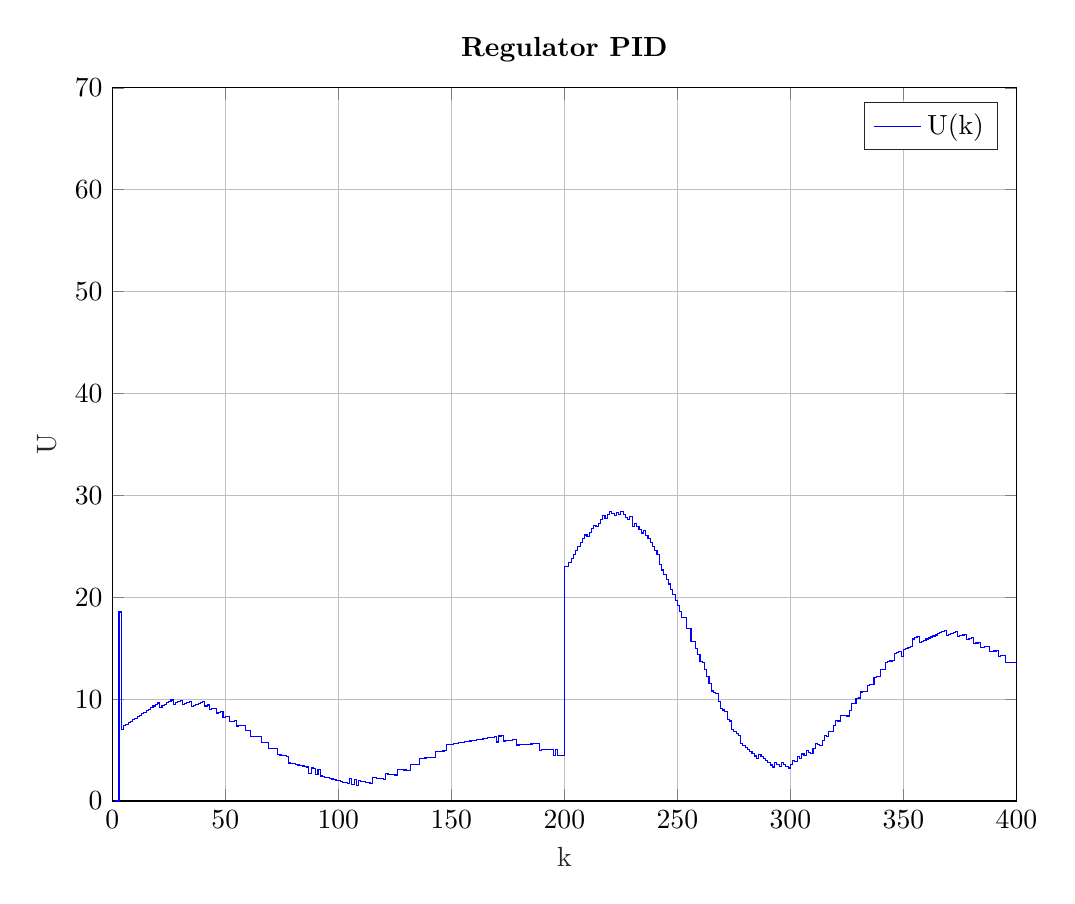
\begin{tikzpicture}

\begin{axis}[%
width=4.521in,
height=3.566in,
at={(0.758in,0.481in)},
scale only axis,
xmin=0,
xmax=400,
xlabel style={font=\color{white!15!black}},
xlabel={k},
ymin=0,
ymax=70,
ylabel style={font=\color{white!15!black}},
ylabel={U},
axis background/.style={fill=white},
title style={font=\bfseries},
title={Regulator PID},
xmajorgrids,
ymajorgrids,
legend style={legend cell align=left, align=left, draw=white!15!black}
]
\addplot[const plot, color=blue] table[row sep=crcr] {%
1	0\\
2	0\\
3	18.56\\
4	6.99999999999999\\
5	7.37499999999999\\
6	7.52499999999999\\
7	7.67499999999999\\
8	7.82499999999999\\
9	7.97499999999998\\
10	8.12499999999998\\
11	8.27499999999998\\
12	8.42499999999998\\
13	8.57499999999998\\
14	8.72499999999998\\
15	8.87499999999998\\
16	9.02499999999997\\
17	9.17499999999997\\
18	9.32499999999997\\
19	9.47499999999997\\
20	9.62499999999997\\
21	9.21819999999998\\
22	9.36699999999998\\
23	9.50499999999997\\
24	9.64299999999997\\
25	9.78099999999997\\
26	9.91899999999997\\
27	9.50019999999995\\
28	9.63699999999994\\
29	9.76299999999994\\
30	9.88899999999994\\
31	9.45819999999995\\
32	9.58299999999995\\
33	9.69699999999994\\
34	9.81099999999994\\
35	9.27539999999994\\
36	9.38799999999993\\
37	9.48799999999993\\
38	9.58799999999993\\
39	9.68799999999993\\
40	9.78799999999993\\
41	9.33119999999994\\
42	9.42999999999993\\
43	8.96119999999991\\
44	9.04799999999991\\
45	9.12399999999991\\
46	8.64319999999992\\
47	8.71799999999992\\
48	8.78199999999992\\
49	8.19639999999992\\
50	8.25899999999992\\
51	8.30899999999992\\
52	7.80219999999993\\
53	7.85099999999993\\
54	7.88899999999993\\
55	7.37019999999991\\
56	7.40699999999991\\
57	7.43299999999991\\
58	7.45899999999991\\
59	6.92819999999992\\
60	6.95299999999992\\
61	6.31739999999991\\
62	6.32999999999991\\
63	6.32999999999991\\
64	6.32999999999991\\
65	6.32999999999991\\
66	5.77319999999993\\
67	5.77199999999993\\
68	5.75999999999993\\
69	5.19119999999991\\
70	5.17799999999991\\
71	5.15399999999991\\
72	5.12999999999991\\
73	4.54919999999992\\
74	4.52399999999992\\
75	4.48799999999992\\
76	4.45199999999992\\
77	4.41599999999992\\
78	3.73039999999992\\
79	3.69299999999992\\
80	3.64299999999992\\
81	3.59299999999992\\
82	3.54299999999992\\
83	3.49299999999992\\
84	3.44299999999992\\
85	3.39299999999992\\
86	3.34299999999992\\
87	2.73619999999993\\
88	3.24179999999992\\
89	3.18099999999992\\
90	2.57419999999994\\
91	3.07979999999993\\
92	2.46219999999994\\
93	2.41099999999994\\
94	2.34899999999994\\
95	2.28699999999994\\
96	2.22499999999994\\
97	2.16299999999994\\
98	2.10099999999994\\
99	2.03899999999995\\
100	1.97699999999995\\
101	1.91499999999995\\
102	1.85299999999995\\
103	1.79099999999995\\
104	1.72899999999995\\
105	2.22379999999994\\
106	1.60619999999995\\
107	2.11179999999994\\
108	1.49419999999995\\
109	1.99979999999994\\
110	1.93899999999994\\
111	1.88899999999994\\
112	1.83899999999994\\
113	1.78899999999995\\
114	1.73899999999995\\
115	2.33859999999995\\
116	2.28999999999995\\
117	2.25399999999995\\
118	2.21799999999995\\
119	2.18199999999995\\
120	2.14599999999995\\
121	2.66679999999994\\
122	2.63199999999994\\
123	2.60799999999994\\
124	2.58399999999994\\
125	2.55999999999994\\
126	3.09279999999996\\
127	3.06999999999996\\
128	3.05799999999996\\
129	3.04599999999996\\
130	3.03399999999996\\
131	3.02199999999996\\
132	3.56679999999995\\
133	3.55599999999995\\
134	3.55599999999995\\
135	3.55599999999995\\
136	4.20559999999995\\
137	4.20699999999995\\
138	4.22099999999995\\
139	4.23499999999996\\
140	4.24899999999996\\
141	4.26299999999996\\
142	4.27699999999996\\
143	4.84779999999994\\
144	4.86299999999994\\
145	4.88899999999994\\
146	4.91499999999994\\
147	4.94099999999994\\
148	5.52379999999996\\
149	5.55099999999996\\
150	5.58899999999996\\
151	5.62699999999996\\
152	5.66499999999996\\
153	5.70299999999996\\
154	5.74099999999996\\
155	5.77899999999996\\
156	5.81699999999996\\
157	5.85499999999996\\
158	5.89299999999996\\
159	5.93099999999996\\
160	5.96899999999996\\
161	6.00699999999996\\
162	6.04499999999996\\
163	6.08299999999996\\
164	6.12099999999996\\
165	6.15899999999997\\
166	6.19699999999997\\
167	6.23499999999997\\
168	6.27299999999997\\
169	6.31099999999997\\
170	5.79219999999995\\
171	6.38579999999997\\
172	6.41299999999997\\
173	5.89419999999994\\
174	5.93099999999994\\
175	5.95699999999994\\
176	5.98299999999994\\
177	6.00899999999994\\
178	6.03499999999994\\
179	5.50419999999995\\
180	5.52899999999995\\
181	5.54299999999995\\
182	5.55699999999996\\
183	5.57099999999996\\
184	5.58499999999996\\
185	5.59899999999996\\
186	5.61299999999996\\
187	5.62699999999996\\
188	5.64099999999996\\
189	5.00539999999995\\
190	5.01799999999995\\
191	5.01799999999995\\
192	5.01799999999995\\
193	5.01799999999995\\
194	5.01799999999995\\
195	4.46119999999997\\
196	5.01679999999995\\
197	4.44919999999997\\
198	4.44799999999997\\
199	4.43599999999997\\
200	22.984\\
201	23.012\\
202	23.4\\
203	23.788\\
204	24.1759999999999\\
205	24.5639999999999\\
206	24.9519999999999\\
207	25.3399999999999\\
208	25.7279999999999\\
209	26.1159999999999\\
210	25.9471999999999\\
211	26.3339999999999\\
212	26.7099999999999\\
213	27.0859999999999\\
214	26.9051999999999\\
215	27.2799999999999\\
216	27.6439999999999\\
217	28.0079999999999\\
218	27.7223999999999\\
219	28.0849999999999\\
220	28.4349999999999\\
221	28.2281999999999\\
222	28.0201999999999\\
223	28.3569999999999\\
224	28.1261999999999\\
225	28.4509999999999\\
226	28.1153999999998\\
227	27.8711999999999\\
228	27.6131999999998\\
229	27.8999999999998\\
230	26.9695999999998\\
231	27.2429999999998\\
232	26.9361999999998\\
233	26.6281999999998\\
234	26.3081999999998\\
235	26.5329999999998\\
236	26.0973999999998\\
237	25.7531999999998\\
238	25.3951999999998\\
239	25.0251999999998\\
240	24.5503999999998\\
241	24.1561999999998\\
242	23.1913999999998\\
243	22.6773999999998\\
244	22.2331999999998\\
245	21.7751999999998\\
246	21.3051999999998\\
247	20.7303999999998\\
248	20.2361999999998\\
249	19.7281999999998\\
250	19.2081999999998\\
251	18.5833999999998\\
252	18.0391999999998\\
253	18.0379999999998\\
254	16.9123999999998\\
255	16.8979999999998\\
256	15.6555999999998\\
257	15.6169999999998\\
258	14.9981999999998\\
259	14.3781999999998\\
260	13.6533999999998\\
261	13.5659999999998\\
262	12.9091999999998\\
263	12.2511999999998\\
264	11.5811999999998\\
265	10.8063999999998\\
266	10.6689999999998\\
267	10.5189999999998\\
268	9.81219999999982\\
269	9.10419999999981\\
270	8.94099999999981\\
271	8.76699999999981\\
272	8.03619999999983\\
273	7.86099999999983\\
274	7.02539999999983\\
275	6.83799999999983\\
276	6.63799999999983\\
277	6.43799999999983\\
278	5.68119999999985\\
279	5.47999999999985\\
280	5.26799999999985\\
281	5.05599999999985\\
282	4.84399999999986\\
283	4.63199999999986\\
284	4.41999999999986\\
285	4.20799999999986\\
286	4.55279999999985\\
287	4.34199999999985\\
288	4.14199999999986\\
289	3.94199999999986\\
290	3.74199999999986\\
291	3.54199999999986\\
292	3.34199999999987\\
293	3.79159999999987\\
294	3.59299999999988\\
295	3.40699999999988\\
296	3.77779999999987\\
297	3.59299999999987\\
298	3.41899999999987\\
299	3.24499999999988\\
300	3.6277999999999\\
301	4.01179999999989\\
302	3.85099999999989\\
303	4.3505999999999\\
304	4.2019999999999\\
305	4.62279999999989\\
306	4.48799999999989\\
307	4.92079999999991\\
308	4.79799999999991\\
309	4.68599999999992\\
310	5.13079999999991\\
311	5.66959999999991\\
312	5.57099999999991\\
313	5.48499999999991\\
314	5.9557999999999\\
315	6.42779999999992\\
316	6.35499999999992\\
317	6.84979999999991\\
318	6.78899999999991\\
319	7.38859999999992\\
320	7.89679999999991\\
321	7.86199999999991\\
322	8.39479999999993\\
323	8.37199999999993\\
324	8.35999999999993\\
325	8.34799999999993\\
326	8.89279999999991\\
327	9.53159999999992\\
328	9.53299999999992\\
329	10.1037999999999\\
330	10.1189999999999\\
331	10.7017999999999\\
332	10.7289999999999\\
333	10.7669999999999\\
334	11.3617999999999\\
335	11.4009999999999\\
336	11.4509999999999\\
337	12.1505999999999\\
338	12.2019999999999\\
339	12.2659999999999\\
340	12.8867999999999\\
341	12.9519999999999\\
342	13.5847999999999\\
343	13.6619999999999\\
344	13.7499999999999\\
345	13.8379999999999\\
346	14.4827999999999\\
347	14.5719999999999\\
348	14.6719999999999\\
349	14.2151999999999\\
350	14.8707999999999\\
351	14.9599999999999\\
352	15.0599999999999\\
353	15.1599999999999\\
354	15.9095999999999\\
355	16.0109999999999\\
356	16.1249999999999\\
357	15.5893999999999\\
358	15.7019999999999\\
359	15.8019999999999\\
360	15.9019999999999\\
361	16.0019999999999\\
362	16.1019999999999\\
363	16.2019999999999\\
364	16.3019999999999\\
365	16.4019999999999\\
366	16.5019999999999\\
367	16.6019999999999\\
368	16.7019999999999\\
369	16.2451999999999\\
370	16.3439999999999\\
371	16.4319999999999\\
372	16.5199999999999\\
373	16.6079999999999\\
374	16.1391999999999\\
375	16.2259999999999\\
376	16.3019999999999\\
377	16.3779999999999\\
378	15.8971999999999\\
379	15.9719999999999\\
380	16.0359999999999\\
381	15.4503999999999\\
382	15.5129999999999\\
383	15.5629999999999\\
384	15.0561999999999\\
385	15.1049999999999\\
386	15.1429999999999\\
387	15.1809999999999\\
388	14.6621999999999\\
389	14.6989999999999\\
390	14.7249999999999\\
391	14.7509999999999\\
392	14.2201999999999\\
393	14.2449999999999\\
394	14.2589999999999\\
395	13.6233999999999\\
396	13.6359999999999\\
397	13.6359999999999\\
398	13.6359999999999\\
399	13.6359999999999\\
400	13.0791999999999\\
};
\addlegendentry{U(k)}

\end{axis}
\end{tikzpicture}%
		\label{w4}
\end{figure}

\begin{figure}

	\centering
	\caption{ }
	% This file was created by matlab2tikz.
%
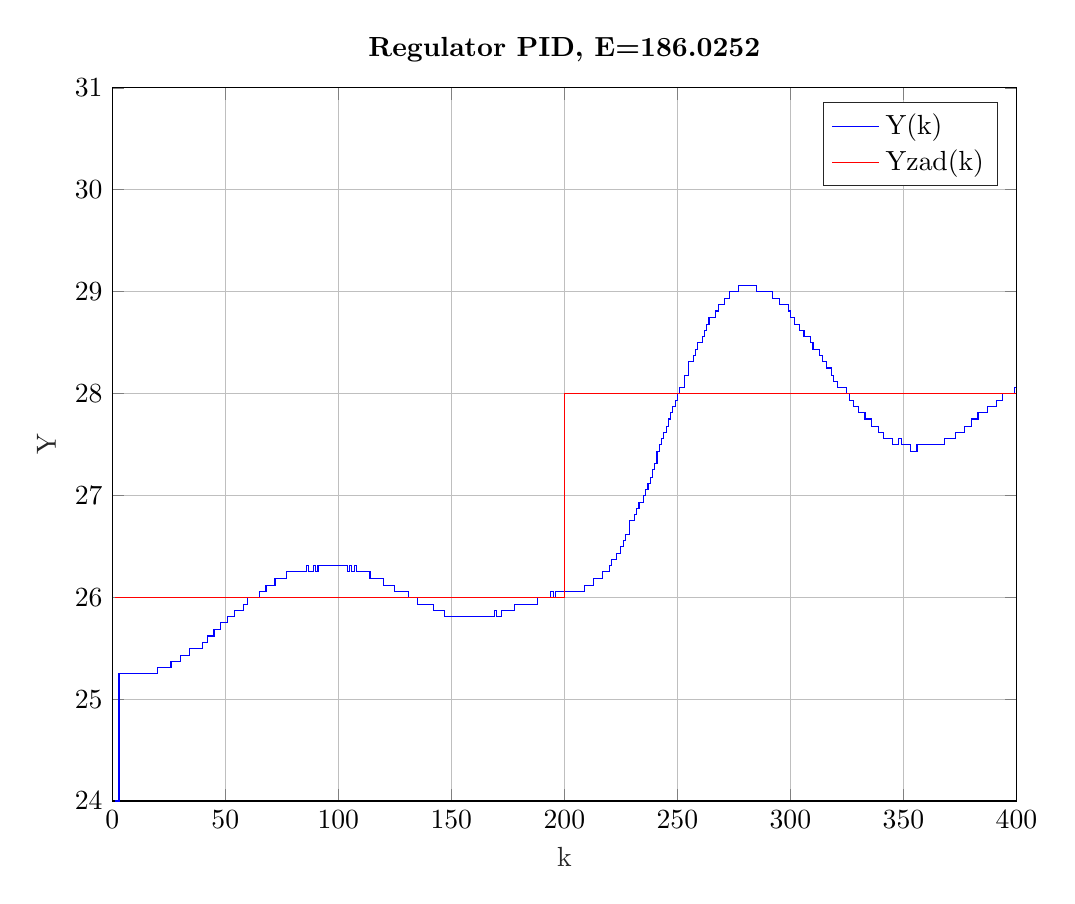
\begin{tikzpicture}

\begin{axis}[%
width=4.521in,
height=3.566in,
at={(0.758in,0.481in)},
scale only axis,
xmin=0,
xmax=400,
xlabel style={font=\color{white!15!black}},
xlabel={k},
ymin=24,
ymax=31,
ylabel style={font=\color{white!15!black}},
ylabel={Y},
axis background/.style={fill=white},
title style={font=\bfseries},
title={Regulator PID, E=186.0252},
xmajorgrids,
ymajorgrids,
legend style={legend cell align=left, align=left, draw=white!15!black}
]
\addplot[const plot, color=blue] table[row sep=crcr] {%
1	24\\
2	24\\
3	25.25\\
4	25.25\\
5	25.25\\
6	25.25\\
7	25.25\\
8	25.25\\
9	25.25\\
10	25.25\\
11	25.25\\
12	25.25\\
13	25.25\\
14	25.25\\
15	25.25\\
16	25.25\\
17	25.25\\
18	25.25\\
19	25.25\\
20	25.31\\
21	25.31\\
22	25.31\\
23	25.31\\
24	25.31\\
25	25.31\\
26	25.37\\
27	25.37\\
28	25.37\\
29	25.37\\
30	25.43\\
31	25.43\\
32	25.43\\
33	25.43\\
34	25.5\\
35	25.5\\
36	25.5\\
37	25.5\\
38	25.5\\
39	25.5\\
40	25.56\\
41	25.56\\
42	25.62\\
43	25.62\\
44	25.62\\
45	25.68\\
46	25.68\\
47	25.68\\
48	25.75\\
49	25.75\\
50	25.75\\
51	25.81\\
52	25.81\\
53	25.81\\
54	25.87\\
55	25.87\\
56	25.87\\
57	25.87\\
58	25.93\\
59	25.93\\
60	26\\
61	26\\
62	26\\
63	26\\
64	26\\
65	26.06\\
66	26.06\\
67	26.06\\
68	26.12\\
69	26.12\\
70	26.12\\
71	26.12\\
72	26.18\\
73	26.18\\
74	26.18\\
75	26.18\\
76	26.18\\
77	26.25\\
78	26.25\\
79	26.25\\
80	26.25\\
81	26.25\\
82	26.25\\
83	26.25\\
84	26.25\\
85	26.25\\
86	26.31\\
87	26.25\\
88	26.25\\
89	26.31\\
90	26.25\\
91	26.31\\
92	26.31\\
93	26.31\\
94	26.31\\
95	26.31\\
96	26.31\\
97	26.31\\
98	26.31\\
99	26.31\\
100	26.31\\
101	26.31\\
102	26.31\\
103	26.31\\
104	26.25\\
105	26.31\\
106	26.25\\
107	26.31\\
108	26.25\\
109	26.25\\
110	26.25\\
111	26.25\\
112	26.25\\
113	26.25\\
114	26.18\\
115	26.18\\
116	26.18\\
117	26.18\\
118	26.18\\
119	26.18\\
120	26.12\\
121	26.12\\
122	26.12\\
123	26.12\\
124	26.12\\
125	26.06\\
126	26.06\\
127	26.06\\
128	26.06\\
129	26.06\\
130	26.06\\
131	26\\
132	26\\
133	26\\
134	26\\
135	25.93\\
136	25.93\\
137	25.93\\
138	25.93\\
139	25.93\\
140	25.93\\
141	25.93\\
142	25.87\\
143	25.87\\
144	25.87\\
145	25.87\\
146	25.87\\
147	25.81\\
148	25.81\\
149	25.81\\
150	25.81\\
151	25.81\\
152	25.81\\
153	25.81\\
154	25.81\\
155	25.81\\
156	25.81\\
157	25.81\\
158	25.81\\
159	25.81\\
160	25.81\\
161	25.81\\
162	25.81\\
163	25.81\\
164	25.81\\
165	25.81\\
166	25.81\\
167	25.81\\
168	25.81\\
169	25.87\\
170	25.81\\
171	25.81\\
172	25.87\\
173	25.87\\
174	25.87\\
175	25.87\\
176	25.87\\
177	25.87\\
178	25.93\\
179	25.93\\
180	25.93\\
181	25.93\\
182	25.93\\
183	25.93\\
184	25.93\\
185	25.93\\
186	25.93\\
187	25.93\\
188	26\\
189	26\\
190	26\\
191	26\\
192	26\\
193	26\\
194	26.06\\
195	26\\
196	26.06\\
197	26.06\\
198	26.06\\
199	26.06\\
200	26.06\\
201	26.06\\
202	26.06\\
203	26.06\\
204	26.06\\
205	26.06\\
206	26.06\\
207	26.06\\
208	26.06\\
209	26.12\\
210	26.12\\
211	26.12\\
212	26.12\\
213	26.18\\
214	26.18\\
215	26.18\\
216	26.18\\
217	26.25\\
218	26.25\\
219	26.25\\
220	26.31\\
221	26.37\\
222	26.37\\
223	26.43\\
224	26.43\\
225	26.5\\
226	26.56\\
227	26.62\\
228	26.62\\
229	26.75\\
230	26.75\\
231	26.81\\
232	26.87\\
233	26.93\\
234	26.93\\
235	27\\
236	27.06\\
237	27.12\\
238	27.18\\
239	27.25\\
240	27.31\\
241	27.43\\
242	27.5\\
243	27.56\\
244	27.62\\
245	27.68\\
246	27.75\\
247	27.81\\
248	27.87\\
249	27.93\\
250	28\\
251	28.06\\
252	28.06\\
253	28.18\\
254	28.18\\
255	28.31\\
256	28.31\\
257	28.37\\
258	28.43\\
259	28.5\\
260	28.5\\
261	28.56\\
262	28.62\\
263	28.68\\
264	28.75\\
265	28.75\\
266	28.75\\
267	28.81\\
268	28.87\\
269	28.87\\
270	28.87\\
271	28.93\\
272	28.93\\
273	29\\
274	29\\
275	29\\
276	29\\
277	29.06\\
278	29.06\\
279	29.06\\
280	29.06\\
281	29.06\\
282	29.06\\
283	29.06\\
284	29.06\\
285	29\\
286	29\\
287	29\\
288	29\\
289	29\\
290	29\\
291	29\\
292	28.93\\
293	28.93\\
294	28.93\\
295	28.87\\
296	28.87\\
297	28.87\\
298	28.87\\
299	28.81\\
300	28.75\\
301	28.75\\
302	28.68\\
303	28.68\\
304	28.62\\
305	28.62\\
306	28.56\\
307	28.56\\
308	28.56\\
309	28.5\\
310	28.43\\
311	28.43\\
312	28.43\\
313	28.37\\
314	28.31\\
315	28.31\\
316	28.25\\
317	28.25\\
318	28.18\\
319	28.12\\
320	28.12\\
321	28.06\\
322	28.06\\
323	28.06\\
324	28.06\\
325	28\\
326	27.93\\
327	27.93\\
328	27.87\\
329	27.87\\
330	27.81\\
331	27.81\\
332	27.81\\
333	27.75\\
334	27.75\\
335	27.75\\
336	27.68\\
337	27.68\\
338	27.68\\
339	27.62\\
340	27.62\\
341	27.56\\
342	27.56\\
343	27.56\\
344	27.56\\
345	27.5\\
346	27.5\\
347	27.5\\
348	27.56\\
349	27.5\\
350	27.5\\
351	27.5\\
352	27.5\\
353	27.43\\
354	27.43\\
355	27.43\\
356	27.5\\
357	27.5\\
358	27.5\\
359	27.5\\
360	27.5\\
361	27.5\\
362	27.5\\
363	27.5\\
364	27.5\\
365	27.5\\
366	27.5\\
367	27.5\\
368	27.56\\
369	27.56\\
370	27.56\\
371	27.56\\
372	27.56\\
373	27.62\\
374	27.62\\
375	27.62\\
376	27.62\\
377	27.68\\
378	27.68\\
379	27.68\\
380	27.75\\
381	27.75\\
382	27.75\\
383	27.81\\
384	27.81\\
385	27.81\\
386	27.81\\
387	27.87\\
388	27.87\\
389	27.87\\
390	27.87\\
391	27.93\\
392	27.93\\
393	27.93\\
394	28\\
395	28\\
396	28\\
397	28\\
398	28\\
399	28.06\\
400	28.06\\
};
\addlegendentry{Y(k)}

\addplot[const plot, color=red] table[row sep=crcr] {%
1	26\\
2	26\\
3	26\\
4	26\\
5	26\\
6	26\\
7	26\\
8	26\\
9	26\\
10	26\\
11	26\\
12	26\\
13	26\\
14	26\\
15	26\\
16	26\\
17	26\\
18	26\\
19	26\\
20	26\\
21	26\\
22	26\\
23	26\\
24	26\\
25	26\\
26	26\\
27	26\\
28	26\\
29	26\\
30	26\\
31	26\\
32	26\\
33	26\\
34	26\\
35	26\\
36	26\\
37	26\\
38	26\\
39	26\\
40	26\\
41	26\\
42	26\\
43	26\\
44	26\\
45	26\\
46	26\\
47	26\\
48	26\\
49	26\\
50	26\\
51	26\\
52	26\\
53	26\\
54	26\\
55	26\\
56	26\\
57	26\\
58	26\\
59	26\\
60	26\\
61	26\\
62	26\\
63	26\\
64	26\\
65	26\\
66	26\\
67	26\\
68	26\\
69	26\\
70	26\\
71	26\\
72	26\\
73	26\\
74	26\\
75	26\\
76	26\\
77	26\\
78	26\\
79	26\\
80	26\\
81	26\\
82	26\\
83	26\\
84	26\\
85	26\\
86	26\\
87	26\\
88	26\\
89	26\\
90	26\\
91	26\\
92	26\\
93	26\\
94	26\\
95	26\\
96	26\\
97	26\\
98	26\\
99	26\\
100	26\\
101	26\\
102	26\\
103	26\\
104	26\\
105	26\\
106	26\\
107	26\\
108	26\\
109	26\\
110	26\\
111	26\\
112	26\\
113	26\\
114	26\\
115	26\\
116	26\\
117	26\\
118	26\\
119	26\\
120	26\\
121	26\\
122	26\\
123	26\\
124	26\\
125	26\\
126	26\\
127	26\\
128	26\\
129	26\\
130	26\\
131	26\\
132	26\\
133	26\\
134	26\\
135	26\\
136	26\\
137	26\\
138	26\\
139	26\\
140	26\\
141	26\\
142	26\\
143	26\\
144	26\\
145	26\\
146	26\\
147	26\\
148	26\\
149	26\\
150	26\\
151	26\\
152	26\\
153	26\\
154	26\\
155	26\\
156	26\\
157	26\\
158	26\\
159	26\\
160	26\\
161	26\\
162	26\\
163	26\\
164	26\\
165	26\\
166	26\\
167	26\\
168	26\\
169	26\\
170	26\\
171	26\\
172	26\\
173	26\\
174	26\\
175	26\\
176	26\\
177	26\\
178	26\\
179	26\\
180	26\\
181	26\\
182	26\\
183	26\\
184	26\\
185	26\\
186	26\\
187	26\\
188	26\\
189	26\\
190	26\\
191	26\\
192	26\\
193	26\\
194	26\\
195	26\\
196	26\\
197	26\\
198	26\\
199	26\\
200	28\\
201	28\\
202	28\\
203	28\\
204	28\\
205	28\\
206	28\\
207	28\\
208	28\\
209	28\\
210	28\\
211	28\\
212	28\\
213	28\\
214	28\\
215	28\\
216	28\\
217	28\\
218	28\\
219	28\\
220	28\\
221	28\\
222	28\\
223	28\\
224	28\\
225	28\\
226	28\\
227	28\\
228	28\\
229	28\\
230	28\\
231	28\\
232	28\\
233	28\\
234	28\\
235	28\\
236	28\\
237	28\\
238	28\\
239	28\\
240	28\\
241	28\\
242	28\\
243	28\\
244	28\\
245	28\\
246	28\\
247	28\\
248	28\\
249	28\\
250	28\\
251	28\\
252	28\\
253	28\\
254	28\\
255	28\\
256	28\\
257	28\\
258	28\\
259	28\\
260	28\\
261	28\\
262	28\\
263	28\\
264	28\\
265	28\\
266	28\\
267	28\\
268	28\\
269	28\\
270	28\\
271	28\\
272	28\\
273	28\\
274	28\\
275	28\\
276	28\\
277	28\\
278	28\\
279	28\\
280	28\\
281	28\\
282	28\\
283	28\\
284	28\\
285	28\\
286	28\\
287	28\\
288	28\\
289	28\\
290	28\\
291	28\\
292	28\\
293	28\\
294	28\\
295	28\\
296	28\\
297	28\\
298	28\\
299	28\\
300	28\\
301	28\\
302	28\\
303	28\\
304	28\\
305	28\\
306	28\\
307	28\\
308	28\\
309	28\\
310	28\\
311	28\\
312	28\\
313	28\\
314	28\\
315	28\\
316	28\\
317	28\\
318	28\\
319	28\\
320	28\\
321	28\\
322	28\\
323	28\\
324	28\\
325	28\\
326	28\\
327	28\\
328	28\\
329	28\\
330	28\\
331	28\\
332	28\\
333	28\\
334	28\\
335	28\\
336	28\\
337	28\\
338	28\\
339	28\\
340	28\\
341	28\\
342	28\\
343	28\\
344	28\\
345	28\\
346	28\\
347	28\\
348	28\\
349	28\\
350	28\\
351	28\\
352	28\\
353	28\\
354	28\\
355	28\\
356	28\\
357	28\\
358	28\\
359	28\\
360	28\\
361	28\\
362	28\\
363	28\\
364	28\\
365	28\\
366	28\\
367	28\\
368	28\\
369	28\\
370	28\\
371	28\\
372	28\\
373	28\\
374	28\\
375	28\\
376	28\\
377	28\\
378	28\\
379	28\\
380	28\\
381	28\\
382	28\\
383	28\\
384	28\\
385	28\\
386	28\\
387	28\\
388	28\\
389	28\\
390	28\\
391	28\\
392	28\\
393	28\\
394	28\\
395	28\\
396	28\\
397	28\\
398	28\\
399	28\\
400	28\\
};
\addlegendentry{Yzad(k)}

\end{axis}
\end{tikzpicture}%
		\label{w5}
\end{figure}

\FloatBarrier
Jak widać regulator PID słabo radzi sobie z regulacją obiektu o tak wolnej dynamice. Wynika to z faktu że operuje on tylko na danych pochodzących bezpośrednio z obiektu i nie może w żaden sposób przewidzieć jego zachowania w przyszłości, dla którego mógłby dostosować wartość sterowania. W takim przypadku lepiej radzi sobie algorytm DMC.

\section{Algorytm DMC}
Następnie zbadano działanie dwóch regulatorów DMC na tym obiekcie. W obu przypadkach uzyto identycznych horyzontów dynamiki i sterowania wynoszących odpowiednio: $N_\mathrm{D}=400$, $N_\mathrm{U}=200$. Przeprowadzono dwa eksperymenty dla różnych wartości lambda: $0.1$ i $1.0$. Efekty przeprowadzonych doświadczeń ukazane są na Rys.~\ref{w6} i ~\ref{w7}.

\begin{figure}

	\centering
	\caption{ }
	% This file was created by matlab2tikz.
%
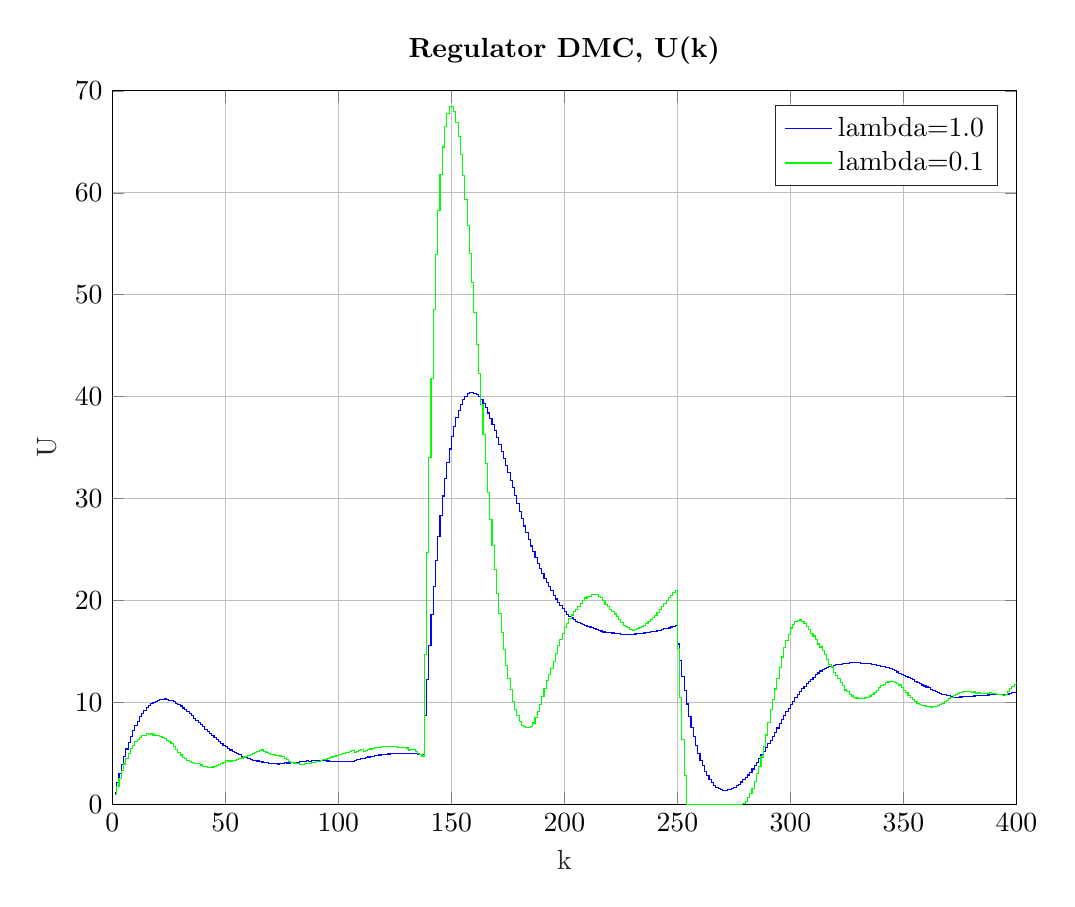
\begin{tikzpicture}

\begin{axis}[%
width=4.521in,
height=3.566in,
at={(0.758in,0.481in)},
scale only axis,
xmin=0,
xmax=400,
xlabel style={font=\color{white!15!black}},
xlabel={k},
ymin=0,
ymax=70,
ylabel style={font=\color{white!15!black}},
ylabel={U},
axis background/.style={fill=white},
title style={font=\bfseries},
title={Regulator DMC, U(k)},
xmajorgrids,
ymajorgrids,
legend style={legend cell align=left, align=left, draw=white!15!black}
]
\addplot[const plot, color=blue] table[row sep=crcr] {%
1	1.08943235571765\\
2	2.09973251410175\\
3	3.03390546721902\\
4	3.89494370157565\\
5	4.68580102004755\\
6	5.40940851661738\\
7	6.06866678543939\\
8	6.66851681878892\\
9	7.21148643542562\\
10	7.70009105035273\\
11	8.13681621766392\\
12	8.58193868174316\\
13	8.91799450837992\\
14	9.20957924154966\\
15	9.45901480358707\\
16	9.6706909773013\\
17	9.84656456603524\\
18	9.99066305588476\\
19	10.1046765222286\\
20	10.1925155538331\\
21	10.2553923854923\\
22	10.2966515851697\\
23	10.3193249288243\\
24	10.266226596263\\
25	10.2046799317454\\
26	10.134607647986\\
27	10.0582546489193\\
28	9.91198786822155\\
29	9.76757537017091\\
30	9.62656898644364\\
31	9.43429548116896\\
32	9.25328148023995\\
33	9.08434472732415\\
34	8.86978174696034\\
35	8.67355366754243\\
36	8.43792891518628\\
37	8.22408012445523\\
38	8.03123898274983\\
39	7.79352298473746\\
40	7.58190549756934\\
41	7.33712230075034\\
42	7.12246611482854\\
43	6.93562694390913\\
44	6.71916950939107\\
45	6.53326567527536\\
46	6.31989393178606\\
47	6.13864724455588\\
48	5.98713640528401\\
49	5.79763609629457\\
50	5.64246241671417\\
51	5.46041192058394\\
52	5.31071473984831\\
53	5.1929457975616\\
54	5.04607609524609\\
55	4.92908271734389\\
56	4.83901678955818\\
57	4.71806734302592\\
58	4.62454231564767\\
59	4.55607396713044\\
60	4.44278428962577\\
61	4.35640991213365\\
62	4.29406865445983\\
63	4.25312818077074\\
64	4.23359109415425\\
65	4.17453116699766\\
66	4.13566548738034\\
67	4.11485529927075\\
68	4.05177902577687\\
69	4.00884165944235\\
70	3.98358062206157\\
71	3.97380574905352\\
72	3.97757328114102\\
73	3.93498727566633\\
74	3.96464832577501\\
75	4.0025777871173\\
76	4.04709506201487\\
77	4.03959440967969\\
78	4.0409775392341\\
79	4.0500344972474\\
80	4.06557944005534\\
81	4.08696532225423\\
82	4.11342125661144\\
83	4.14424860957347\\
84	4.17794848039379\\
85	4.21471874809964\\
86	4.25209627087702\\
87	4.22180587753698\\
88	4.26386618596653\\
89	4.23807634688306\\
90	4.28212511594438\\
91	4.32429486900001\\
92	4.29663990399058\\
93	4.27245730246123\\
94	4.25134770290935\\
95	4.2312814328937\\
96	4.21305925115925\\
97	4.19687654819682\\
98	4.18321428791685\\
99	4.17192881738074\\
100	4.16372338880858\\
101	4.15672317913826\\
102	4.15120239768166\\
103	4.14757488626453\\
104	4.14603802858266\\
105	4.21528591009448\\
106	4.21297965347191\\
107	4.27987367986385\\
108	4.34398644447824\\
109	4.40572125819102\\
110	4.46377257152693\\
111	4.51876266047355\\
112	4.57191013754136\\
113	4.62142641374353\\
114	4.66807783579356\\
115	4.71314805250552\\
116	4.75463764808529\\
117	4.79134544973577\\
118	4.82490114736741\\
119	4.85409695093008\\
120	4.88025963733876\\
121	4.90187820012776\\
122	4.92058269298862\\
123	4.93526309567313\\
124	4.94761184142996\\
125	4.95620045579116\\
126	4.9606885324982\\
127	4.96253665169094\\
128	4.96299945421184\\
129	4.96172133848907\\
130	4.95933230318011\\
131	4.95569165215981\\
132	4.94957301292259\\
133	4.94035664277152\\
134	4.92782885011105\\
135	4.91376836843491\\
136	4.89733643831792\\
137	4.87815478177116\\
138	8.71482066425099\\
139	12.2705671964488\\
140	15.5575346961528\\
141	18.5852539640305\\
142	21.3658697227182\\
143	23.9092328939794\\
144	26.2248381103634\\
145	28.3314856374397\\
146	30.238204545256\\
147	31.9549277123099\\
148	33.4898983897594\\
149	34.8530910285511\\
150	36.0542680365064\\
151	37.1008973091043\\
152	37.9344374664661\\
153	38.6419197263351\\
154	39.2292383368812\\
155	39.7089869722872\\
156	40.0310425863887\\
157	40.2702137549314\\
158	40.3738534947516\\
159	40.4144470263366\\
160	40.3411994597592\\
161	40.2196497230087\\
162	39.9994963823498\\
163	39.6962055268639\\
164	39.3205235416186\\
165	38.889259324462\\
166	38.393595171526\\
167	37.8533966617516\\
168	37.2828228295678\\
169	36.6877444971647\\
170	36.0088105364972\\
171	35.3222395241807\\
172	34.6416843301003\\
173	33.9598372172127\\
174	33.2305491191559\\
175	32.51828811815\\
176	31.7645800451908\\
177	31.0405027007988\\
178	30.27727464343\\
179	29.4962911153205\\
180	28.7586281348075\\
181	28.0014636818858\\
182	27.2938384367176\\
183	26.6386946921065\\
184	25.9633821026977\\
185	25.336238998982\\
186	24.7618728226672\\
187	24.1755516562175\\
188	23.6450136979027\\
189	23.096253381073\\
190	22.6032757145069\\
191	22.1587676104864\\
192	21.7560503928071\\
193	21.321288493814\\
194	20.9311762651908\\
195	20.5114154701353\\
196	20.1296857554033\\
197	19.7809102415797\\
198	19.4667326327509\\
199	19.1708485670087\\
200	18.8986164172619\\
201	18.6519512260755\\
202	18.4248531319265\\
203	18.2708066163879\\
204	18.1134053281543\\
205	17.9586591140859\\
206	17.8110399496819\\
207	17.7250047838519\\
208	17.6334871050002\\
209	17.5243691444051\\
210	17.4642230214328\\
211	17.3885435506055\\
212	17.2952774860033\\
213	17.241134737488\\
214	17.1659855845872\\
215	17.059257398608\\
216	16.9883574493201\\
217	16.8910273566652\\
218	16.8846082809661\\
219	16.8468636531371\\
220	16.8362852845024\\
221	16.7912495011141\\
222	16.7720443175674\\
223	16.76735703839\\
224	16.7181956477357\\
225	16.6851957705464\\
226	16.6681909773133\\
227	16.6587470602481\\
228	16.6571944980832\\
229	16.6634255251209\\
230	16.6768323064261\\
231	16.69711041783\\
232	16.7168827870566\\
233	16.7398747107172\\
234	16.7646594286029\\
235	16.7941876754751\\
236	16.828195676363\\
237	16.867011946619\\
238	16.9047305107746\\
239	16.9424084006398\\
240	16.9814652574817\\
241	17.0226996558312\\
242	17.0681414981052\\
243	17.1111298820546\\
244	17.2107825876063\\
245	17.2491936207775\\
246	17.2902677622709\\
247	17.3847653114299\\
248	17.4749561643462\\
249	17.5621713238715\\
250	15.7149614106748\\
251	14.0623720867649\\
252	12.5368304528928\\
253	11.1300603300002\\
254	9.83236944961992\\
255	8.64333676162557\\
256	7.55382214212722\\
257	6.61669631343192\\
258	5.76367572186346\\
259	4.99531050892193\\
260	4.30283012472376\\
261	3.75409507983472\\
262	3.20100346263838\\
263	2.77651994056197\\
264	2.41081726072416\\
265	2.10102945734359\\
266	1.8400367053033\\
267	1.62625080927693\\
268	1.51159170203573\\
269	1.42418410299256\\
270	1.36073349316794\\
271	1.37337492183836\\
272	1.39896008432173\\
273	1.43446663208358\\
274	1.52809840902919\\
275	1.62812586231487\\
276	1.79645494654827\\
277	1.95884554607332\\
278	2.17356192112069\\
279	2.38079888945644\\
280	2.63004027622514\\
281	2.85864059857085\\
282	3.12913683510608\\
283	3.44342285082797\\
284	3.79012293707711\\
285	4.10467871336492\\
286	4.4505442875338\\
287	4.83197357426532\\
288	5.17730128521189\\
289	5.56051461253553\\
290	5.90844811401135\\
291	6.27499233831968\\
292	6.65640205233212\\
293	7.05376924601687\\
294	7.47219532201679\\
295	7.90211178973436\\
296	8.28450515457096\\
297	8.6692682448234\\
298	9.05853289784983\\
299	9.38769571411497\\
300	9.73500422227026\\
301	10.0874985912942\\
302	10.4392129274339\\
303	10.7305236054782\\
304	11.022891982533\\
305	11.324642062734\\
306	11.5632173243316\\
307	11.8074898968244\\
308	12.054256168339\\
309	12.2536124268849\\
310	12.4620653672882\\
311	12.6886192500607\\
312	12.8708350427768\\
313	13.065915884625\\
314	13.2163316559267\\
315	13.3247217472976\\
316	13.3915357679124\\
317	13.4859858469095\\
318	13.5428517437042\\
319	13.6230436306764\\
320	13.6676550419818\\
321	13.6818237645209\\
322	13.7343978170941\\
323	13.762902961779\\
324	13.7692832728444\\
325	13.8233559919031\\
326	13.8621349133822\\
327	13.8856433606962\\
328	13.8951833105686\\
329	13.8908125652543\\
330	13.8719689991304\\
331	13.8448780395431\\
332	13.8122798344148\\
333	13.7784727120551\\
334	13.8017003743428\\
335	13.762660693118\\
336	13.7243378261411\\
337	13.6834628668105\\
338	13.6387197312708\\
339	13.5937610557034\\
340	13.5488987879359\\
341	13.5022341985522\\
342	13.4529620171141\\
343	13.4009330637179\\
344	13.2904211902071\\
345	13.1816934112823\\
346	13.0738257749142\\
347	12.965922755377\\
348	12.856612557952\\
349	12.7470673536032\\
350	12.6393961312057\\
351	12.5401356789236\\
352	12.447126738998\\
353	12.3579988869286\\
354	12.2041245217529\\
355	12.0571770995532\\
356	11.9246940271932\\
357	11.803793976837\\
358	11.6922420369484\\
359	11.5906024951362\\
360	11.4968818323754\\
361	11.408209729673\\
362	11.2687091435119\\
363	11.1443619650181\\
364	11.0332320361712\\
365	10.935713595929\\
366	10.8539932480092\\
367	10.7842437329577\\
368	10.7269335173444\\
369	10.6779870958257\\
370	10.6460900524658\\
371	10.5614685921774\\
372	10.4938618768452\\
373	10.4972458730716\\
374	10.5019693131648\\
375	10.5149340091304\\
376	10.53120128002\\
377	10.5477544510194\\
378	10.5653705413711\\
379	10.5808723171802\\
380	10.5976584355634\\
381	10.6142527430253\\
382	10.6315364394064\\
383	10.6498597521352\\
384	10.6657657746527\\
385	10.6812380089908\\
386	10.696168384359\\
387	10.7147610987227\\
388	10.7372164874959\\
389	10.7515661168759\\
390	10.7677916866985\\
391	10.7825992495175\\
392	10.738261927515\\
393	10.75568253956\\
394	10.769850118603\\
395	10.790676538971\\
396	10.8106147553585\\
397	10.833227182278\\
398	10.9127150310866\\
399	10.9258100336747\\
400	10.9361900709524\\
};
\addlegendentry{lambda=1.0}

\addplot[const plot, color=green] table[row sep=crcr] {%
1	0.947571322192094\\
2	1.77307622193301\\
3	2.4850187131778\\
4	3.26940183531681\\
5	3.93361868091282\\
6	4.48699563414921\\
7	4.93855843684505\\
8	5.48003610964998\\
9	5.74014839259286\\
10	6.10555820357739\\
11	6.38328086851864\\
12	6.58072458036207\\
13	6.70538919205997\\
14	6.7644111676892\\
15	6.94304925944515\\
16	6.87385264003152\\
17	6.94252039631442\\
18	6.7807735665041\\
19	6.77210081491401\\
20	6.72514181834386\\
21	6.64334351551944\\
22	6.53588747052477\\
23	6.41062110126801\\
24	6.26708792857365\\
25	6.11992244006348\\
26	5.96704577309598\\
27	5.63655067974425\\
28	5.33758863486646\\
29	5.06511807035026\\
30	4.82127367926284\\
31	4.61051652943691\\
32	4.43462591110883\\
33	4.28660825596851\\
34	4.17027024258146\\
35	4.08543083350248\\
36	4.03022894056767\\
37	4.00090142191376\\
38	3.99509272645522\\
39	3.83834535454301\\
40	3.72386079955734\\
41	3.64919804073563\\
42	3.61391733889281\\
43	3.61026956931471\\
44	3.63874117871419\\
45	3.69329421407195\\
46	3.77334827295875\\
47	3.87188899842061\\
48	3.98306426270151\\
49	4.11118296040761\\
50	4.25406316839878\\
51	4.22874856062912\\
52	4.22950388333705\\
53	4.26088375441003\\
54	4.31001133450752\\
55	4.37396592463489\\
56	4.44772560969442\\
57	4.53198082465127\\
58	4.62118477514811\\
59	4.70988204552686\\
60	4.80065383449814\\
61	4.89051901665198\\
62	4.97951564933871\\
63	5.06403925813125\\
64	5.1514224960467\\
65	5.23463697348561\\
66	5.3116470175057\\
67	5.17674198731905\\
68	5.0605643016602\\
69	4.96667064798413\\
70	4.88952266102866\\
71	4.82986019551893\\
72	4.78257381327829\\
73	4.74770570882872\\
74	4.72177724105036\\
75	4.70339992478554\\
76	4.5147522004927\\
77	4.35561557884087\\
78	4.22429325839071\\
79	4.11961758592339\\
80	4.04015047711275\\
81	3.98375087573468\\
82	3.94843825037639\\
83	3.93241803739942\\
84	3.9322726570586\\
85	3.94954637868687\\
86	3.97544700741837\\
87	4.01112854602924\\
88	4.05625539492723\\
89	4.10863905180311\\
90	4.16408873793951\\
91	4.22237559266955\\
92	4.28558775431972\\
93	4.35205438351894\\
94	4.42305774790396\\
95	4.4915982627343\\
96	4.56043926882512\\
97	4.62933057252775\\
98	4.70002648225189\\
99	4.77197528645736\\
100	4.8439949602959\\
101	4.9132900116571\\
102	4.97889963131889\\
103	5.04389730421258\\
104	5.10686775532763\\
105	5.17121112596099\\
106	5.23066024869625\\
107	5.10945281684616\\
108	5.18470521572637\\
109	5.25683464900561\\
110	5.32082178297141\\
111	5.20085074066331\\
112	5.28031632694596\\
113	5.35057725002909\\
114	5.41432483067042\\
115	5.47291413157637\\
116	5.52392495676893\\
117	5.56248810951755\\
118	5.59677120591107\\
119	5.6192776654999\\
120	5.63269808418485\\
121	5.63983772658964\\
122	5.64160966386901\\
123	5.63696401178441\\
124	5.62767831776721\\
125	5.61500903132679\\
126	5.59188979661807\\
127	5.57007288783818\\
128	5.54910921855179\\
129	5.52865917635694\\
130	5.51094619624706\\
131	5.31626723713485\\
132	5.32077577487878\\
133	5.32203631776173\\
134	5.14326502440085\\
135	4.98410510096144\\
136	4.84653610684341\\
137	4.72450832309537\\
138	14.7245083230954\\
139	24.7245083230954\\
140	34.0100210316093\\
141	41.7748208787414\\
142	48.5055609944994\\
143	53.9156660784354\\
144	58.2978155089235\\
145	61.8018955393749\\
146	64.5032054938743\\
147	66.4789630404482\\
148	67.7867944661229\\
149	68.4938395228877\\
150	68.4796489046539\\
151	68.0035942676543\\
152	66.911268348504\\
153	65.5409066817996\\
154	63.7544648284921\\
155	61.6581782766739\\
156	59.3020431903992\\
157	56.7572517648928\\
158	54.0763745470133\\
159	51.160819651211\\
160	48.2340102409057\\
161	45.156661018493\\
162	42.2430311318706\\
163	39.2632350577825\\
164	36.3001797373475\\
165	33.420257902494\\
166	30.6257502244797\\
167	27.9142300940613\\
168	25.3947946672099\\
169	23.0379700155184\\
170	20.6852541012129\\
171	18.7273726002602\\
172	16.807896022075\\
173	15.1383654719617\\
174	13.649714231541\\
175	12.347447671162\\
176	11.2299161801743\\
177	10.1156425953807\\
178	9.30519263015992\\
179	8.66080877478787\\
180	8.11144403390482\\
181	7.70818945824215\\
182	7.58447573386109\\
183	7.52106424625819\\
184	7.50172863398716\\
185	7.63628194682523\\
186	7.96160609229408\\
187	8.47915959131414\\
188	9.12864015377513\\
189	9.81431514197399\\
190	10.5746276207531\\
191	11.3517262601828\\
192	12.0968564245634\\
193	12.7316211086671\\
194	13.3260543511333\\
195	14.0244174031941\\
196	14.7735949806744\\
197	15.5295584462596\\
198	16.1401517922999\\
199	16.7544394190206\\
200	17.3513904062389\\
201	17.7721584541608\\
202	18.1842510606176\\
203	18.5663564708562\\
204	18.8882681058799\\
205	19.1372744326617\\
206	19.3647442940467\\
207	19.7348248949949\\
208	20.0271403766451\\
209	20.2345356708675\\
210	20.361545538175\\
211	20.4027284621762\\
212	20.5420926481381\\
213	20.5756082411442\\
214	20.533680637835\\
215	20.4173888943619\\
216	20.2458609025545\\
217	20.0256121560529\\
218	19.5975788423698\\
219	19.3611000034379\\
220	19.1206228341669\\
221	18.8827515797496\\
222	18.6616655066773\\
223	18.409407970314\\
224	18.1312425413395\\
225	17.8423328821655\\
226	17.5707539357125\\
227	17.4472638499911\\
228	17.3031929549916\\
229	17.1613033303458\\
230	17.0405626235202\\
231	17.1671800001103\\
232	17.2535067521649\\
233	17.3317749831252\\
234	17.415903419287\\
235	17.5322007546328\\
236	17.6891025919744\\
237	17.8957540319927\\
238	18.1034050508979\\
239	18.3211329254108\\
240	18.5546017805793\\
241	18.811867585116\\
242	19.1132074873475\\
243	19.401712884441\\
244	19.6830016980858\\
245	19.9638343283277\\
246	20.2589914221828\\
247	20.5147946799384\\
248	20.7525930340466\\
249	20.9932244232401\\
250	15.2723562438025\\
251	10.470562996839\\
252	6.34365093564394\\
253	2.80654144210113\\
254	0\\
255	0\\
256	0\\
257	0\\
258	0\\
259	0\\
260	0\\
261	0\\
262	0\\
263	0\\
264	0\\
265	0\\
266	0\\
267	0\\
268	0\\
269	0\\
270	0\\
271	0\\
272	0\\
273	0\\
274	0\\
275	0\\
276	0\\
277	0\\
278	0\\
279	0.0571213954300641\\
280	0.286691789244031\\
281	0.659565121559635\\
282	1.02156544480024\\
283	1.52265806483873\\
284	2.19423361232109\\
285	2.97245175855863\\
286	3.70329950470846\\
287	4.62084319238066\\
288	5.62762973454054\\
289	6.78708378208594\\
290	8.02365020322869\\
291	9.25156026120307\\
292	10.2667799447666\\
293	11.2986141126517\\
294	12.3517446184463\\
295	13.3993914084567\\
296	14.439038940549\\
297	15.3826835554011\\
298	16.0703666180681\\
299	16.6915175436991\\
300	17.2832349306336\\
301	17.6532839142768\\
302	17.9543343764621\\
303	18.0266612973611\\
304	18.0760812942921\\
305	17.9214179798099\\
306	17.7471316501257\\
307	17.4233228362243\\
308	17.1417354029446\\
309	16.7824789429493\\
310	16.4990316058213\\
311	16.1259322700966\\
312	15.7188601160575\\
313	15.4231329280181\\
314	15.0598390799306\\
315	14.646146474065\\
316	14.1712073297004\\
317	13.7161143889886\\
318	13.4590571910039\\
319	12.9620395736438\\
320	12.6652465789844\\
321	12.3393565423397\\
322	11.9800228065103\\
323	11.6724193138509\\
324	11.199024773992\\
325	11.0630093243941\\
326	10.7979913272503\\
327	10.6173876149897\\
328	10.4974668218364\\
329	10.4132912480864\\
330	10.3432997417884\\
331	10.3303821422605\\
332	10.3643155698189\\
333	10.4915883449528\\
334	10.5045277157531\\
335	10.6121631695172\\
336	10.7820685493748\\
337	10.9805769940667\\
338	11.1811841585049\\
339	11.4049456625125\\
340	11.6118195752601\\
341	11.7819828783163\\
342	11.910714369664\\
343	11.9884815783421\\
344	12.0333503834967\\
345	12.0322720046447\\
346	11.9758187170231\\
347	11.8628826821643\\
348	11.6898171693969\\
349	11.442677008764\\
350	11.1696602040823\\
351	10.9214616688675\\
352	10.6958775471833\\
353	10.4790062454263\\
354	10.2547208772904\\
355	10.0299880532494\\
356	9.86683635279752\\
357	9.75127138141694\\
358	9.6721947635565\\
359	9.63959482039401\\
360	9.60756158909752\\
361	9.5662428331851\\
362	9.53510577127027\\
363	9.55645300436107\\
364	9.59309543919171\\
365	9.66611552431993\\
366	9.78844389116248\\
367	9.91168798313525\\
368	10.0475017308285\\
369	10.1741824196274\\
370	10.3553685672193\\
371	10.4852001882377\\
372	10.6436301194401\\
373	10.7907936468732\\
374	10.8878876916423\\
375	10.9856229662892\\
376	11.062504772794\\
377	11.0925635702374\\
378	11.0947739798767\\
379	11.0359972183923\\
380	10.9374137963063\\
381	11.0056520782369\\
382	10.8850488142625\\
383	10.9575045188147\\
384	10.8182354225196\\
385	10.8556126994213\\
386	10.873091463148\\
387	10.8916323956904\\
388	10.9242944313284\\
389	10.8893692406045\\
390	10.8569477480902\\
391	10.8010943667991\\
392	10.759216012831\\
393	10.7297156708142\\
394	10.7002194736221\\
395	10.7388989350828\\
396	11.0182147704222\\
397	11.3070544925101\\
398	11.5675522621883\\
399	11.7779649703889\\
400	11.9535929623009\\
};
\addlegendentry{lambda=0.1}

\end{axis}
\end{tikzpicture}%
		\label{w6}
\end{figure}

\begin{figure}

	\centering
	\caption{ }
	\input{./PLOTS/DMC_Y.tex}
		\label{w7}
\end{figure}

\FloatBarrier
Jak widać, algorytm DMC radzi sobie znacznie lepiej przy sterowaniu obiektem o wolniejszej dynamice, niż algorytm PID. Wynika to z faktu iż DMC posługuje się modelem obiektu w postaci odpowiedzi skokowej, dzięki czemu może on przewidzieć zachowanie się obieku w danej sytuacji i odpowiednio wcześniej reagować, zmieniając wartości sterowania, przez co osaiąga on wartość zadaną w znacznie szybszy i stabilniejszy sposób niż PID.